\documentclass[11pt]{article}

\usepackage[margin=1in]{geometry}
\usepackage{amsmath, amssymb}
\usepackage{booktabs}
\usepackage{setspace}
\usepackage[hidelinks]{hyperref}
\usepackage{enumitem}
\usepackage{graphicx}
\usepackage[font=small]{caption}
\graphicspath{{./}{../design2/}}

\title{The Local Housing-Market Effects of Act 22/60 Investor Purchases:\\
Data and Empirical Design}
\author{}
\date{August 2026}

\newcommand{\pcth}{\texttt{pcthispanic}}

\begin{document}
\maketitle
\onehalfspacing

\section{Research question}

When a tax-incentivized migrant (an Act 22/60 ``Individual Investor'' decree
holder) buys a residential property in Puerto Rico, what happens to the housing
market immediately around that property --- to prices, and to who transacts?

\section{Data construction}

\subsection{Identifying investor properties}

\begin{itemize}[leftmargin=*]
  \item \textbf{Decree holders.} Government lists of individual grantees:
  3{,}181 (Act 22) and 2{,}672 (Act 60) names; 5{,}770 distinct first--last
  pairs pooled.
  \item \textbf{CRIM cadastral registry.} Name searches against the CRIM parcel
  layer (via its ArcGIS REST service) matched 26{,}673 unique parcels, each with
  full attributes, centroid coordinates, and the parcel's \emph{most recent}
  sale (price, date, buyer, seller). CRIM stores only the latest transaction
  per parcel.
  \item \textbf{Karibe property registry.} Registry name-search results;
  cadastral numbers extracted from registral descriptions and resolved in CRIM
  provide a second, largely non-overlapping source.
  \item \textbf{Match confidence.} Name$\to$parcel matching is noisy for common
  names. A name returning \emph{exactly one} property is treated as
  high-confidence (``unique match''): 810 parcels via CRIM, 755 via Karibe
  (surname-validated, geocoded), union \textbf{1{,}306 parcels} (259
  cross-validated in both). The event studies use this base.
  \item \textbf{Coverage.} High-confidence identification covers 22.5\% of
  searched names (26.7\% including a validated multi-match recovery tier),
  versus 49--61\% declared homeownership in the Act 22 annual reports. The gap
  is dominated by LLC/trust purchases (invisible to name search), name-format
  failures, and registry availability; the identified sample skews toward
  single-property, personal-name buyers.
\end{itemize}

\subsection{Events}

An \textbf{event} is a dated investor purchase: unique-match parcels with a
valid CRIM sale date, collapsing same-day, same-location purchases (condo units
bought together) into one event, giving 1{,}256 events (1{,}200 in the decree
era, $\geq 2012$, used in estimation). Purchases cluster heavily: the median
event has 25 other events within 1\,km (158 are fully isolated), so
contamination is measured per event and used in robustness.

\subsection{Outcomes: nearby sales}

For each event, every CRIM parcel within 1{,}000\,m with a recorded sale:
3.47M sale$\times$event pairs over 328K distinct parcels, each carrying
distance, sale price/date/parties, property characteristics (lot size, assessed
structure value, condo-unit and vacant-land indicators), and 2020 census tract.
\emph{Rings:} 0--250\,m (treated), 250--400\,m (buffer, dropped), 400--1{,}000\,m
(control). \emph{Filters:} nominal transfers ($<\$10$k), implausible dates, and
sales of investor-matched parcels are excluded. \emph{Caveat:} CRIM keeps only
each parcel's last sale, so earlier sales are censored by later resales; the
within-window, near-versus-far design mitigates this, and Figure~5 tests it.

\subsection{Placebo events}

1{,}500 purchases by non-corporate \emph{individual} buyers in the investor
price band (\$285K--\$3.9M, the p25--p95 of investor purchases), located within
250\,m of a real event site (where the sales pool has full coverage) but more
than three years apart in time. Far rings are truncated at 750\,m for both the
placebo run and a matched real-event baseline.

\subsection{Buyer/seller origin proxy}

Party names are classified against the Census 2010 surnames file (\pcth),
taking the maximum across name tokens (robust to CRIM's inconsistent name
ordering; appropriate under the Puerto Rican two-surname convention). Names
with $\pcth \leq 20$ are ``non-Hispanic-named'' (mainland proxy), $\geq 70$
``Hispanic-named'' (local proxy); corporate, ambiguous, and unmatched names are
left unclassified, and the raw score is retained for re-thresholding.
\emph{Validity:} 67\% of investor purchases have non-Hispanic-named buyers
versus 10\% of surrounding market sales. \emph{Caveat:} the proxy captures
\emph{name} origin --- stateside Puerto Ricans and other Hispanic-named
mainlanders classify as local, so mainland penetration and displacement effects
are understated.

\section{Empirical design}

\subsection{Panel construction}

Because CRIM records one (the last) sale per parcel, sales are aggregated into
an event$\times$ring$\times$period panel. Let $e$ index events, $r \in
\{\text{near}, \text{far}\}$ rings, and $t$ calendar periods (years in the
robustness suite). The cell outcome is the mean log price among the
$N_{ert}$ transactions in cell $(e,r)$ in period $t$:
\begin{equation}
  \bar{y}_{ert} \;=\; \frac{1}{N_{ert}} \sum_{j \in (e,r,t)} \ln P_{j},
\end{equation}
where $P_j$ is the sale price of transaction $j$. Treatment is absorbing and
turns on for the near cell in the event period $t_e$:
\begin{equation}
  D_{ert} \;=\; \mathbf{1}\{r = \text{near}\}\times \mathbf{1}\{t \geq t_e\},
\end{equation}
so far cells are never treated and serve as clean controls. In the
tract-fixed-effects specification, $\ln P_j$ is first residualized on census
tract dummies at the sale level ($\ln P_j - \hat{\gamma}_{\tau(j)}$) and the
residual is aggregated instead; results are unchanged.

\subsection{Local projections difference-in-differences (LP-DiD)}

Following Dube, Girardi, Jord\`a and Taylor (2023), the dynamic effect at each
horizon $h$ is estimated from a separate long-difference regression on the
stacked cell panel. For post-treatment horizons $h = 0, 1, \dots, H$:
\begin{equation}
  \bar{y}_{er,\,t+h} - \bar{y}_{er,\,t-1}
  \;=\;
  \beta_h^{\text{LP-DiD}}\, \Delta D_{ert}
  \;+\; \delta_t^{h}
  \;+\; \varepsilon_{ert}^{h},
  \label{eq:lpdid_post}
\end{equation}
and for pre-treatment horizons $h = 2, \dots, Q$ (with $h=1$ the normalization):
\begin{equation}
  \bar{y}_{er,\,t-h} - \bar{y}_{er,\,t-1}
  \;=\;
  \beta_{-h}^{\text{LP-DiD}}\, \Delta D_{ert}
  \;+\; \delta_t^{h}
  \;+\; \varepsilon_{ert}^{h},
  \label{eq:lpdid_pre}
\end{equation}
where $\Delta D_{ert} = D_{ert} - D_{er,t-1}$ indicates that the near cell of
event $e$ enters treatment in period $t$, and $\delta_t^h$ are
horizon-specific calendar-period effects.

Each horizon-$h$ regression is estimated on the restricted ``clean'' sample
\begin{equation}
  \Big\{\, (e,r,t) : \underbrace{\Delta D_{ert} = 1}_{\text{newly treated near cells}}
  \;\;\text{or}\;\;
  \underbrace{D_{er,s} = 0 \;\; \forall s}_{\text{never-treated far cells}} \Big\},
\end{equation}
which is the \texttt{nevertreated} option: the counterfactual change
$\bar{y}_{er,t+h} - \bar{y}_{er,t-1}$ for a newly treated near cell is
identified from far cells over the same calendar window, and no
already-treated observation is ever used as a control (the negative-weighting
problem of two-way fixed effects under staggered timing cannot arise).
$\beta_h^{\text{LP-DiD}}$ is a variance-weighted average of event-specific
effects; standard errors are clustered by cell. The identifying assumption is
within-micro-neighborhood parallel trends: absent the purchase, prices of homes
transacting 0--250\,m from the site would have evolved like those
400--1{,}000\,m away, conditional on calendar-time effects --- shocks common to
the micro-area (Hurricane Mar\'ia, the 2020--21 in-migration wave) difference
out by construction, and equations~\eqref{eq:lpdid_pre} provide the testable
pre-trend restrictions $\beta_{-h} = 0$.

Two scope conditions follow from the ring structure. First, the near--far
contrast differences out any effect \emph{common to the full 1-km
neighborhood}: the design identifies the hyper-local increment around a
purchase site, not the neighborhood-level effect of aggregate investor
inflows, which requires the complementary tract-level staggered design using
the tract$\times$month price panel (Section~\ref{sec:design2}). Second,
because purchases cluster at the enclave scale, other investor purchases in
dense areas fall disproportionately inside the near ring itself; the
estimated contrast there measures the cumulative local dose of investor
activity rather than the effect of a single purchase (see
Figure~\ref{fig:dose}).

\subsection{Robustness to the estimation approach}

The cell-mean panel is a construction choice; the ring literature
(Linden and Rockoff 2008; Campbell, Giglio and Pathak 2011) instead estimates
on individual transactions: stacked sale-level regressions of log price on
near$\times$post (or near$\times$event-time dummies) with event$\times$ring
and event$\times$calendar-year fixed effects, standard errors clustered by
event. The two implementations also weight differently --- transactions
versus events --- so agreement is informative rather than mechanical.
Re-estimating the baseline this way yields a pooled near$\times$post effect
of $+7.09$ log points (s.e.\ $1.58$), and $+6.72$ ($1.32$) with hedonic
controls (log lot size, sub-unit and vacant-land indicators), against the
cell-level LP-DiD baseline of $+6.95$ ($1.81$); the event-study paths
coincide horizon by horizon (Figure~\ref{fig:salelevel}).

\begin{figure}[htbp]
  \centering
  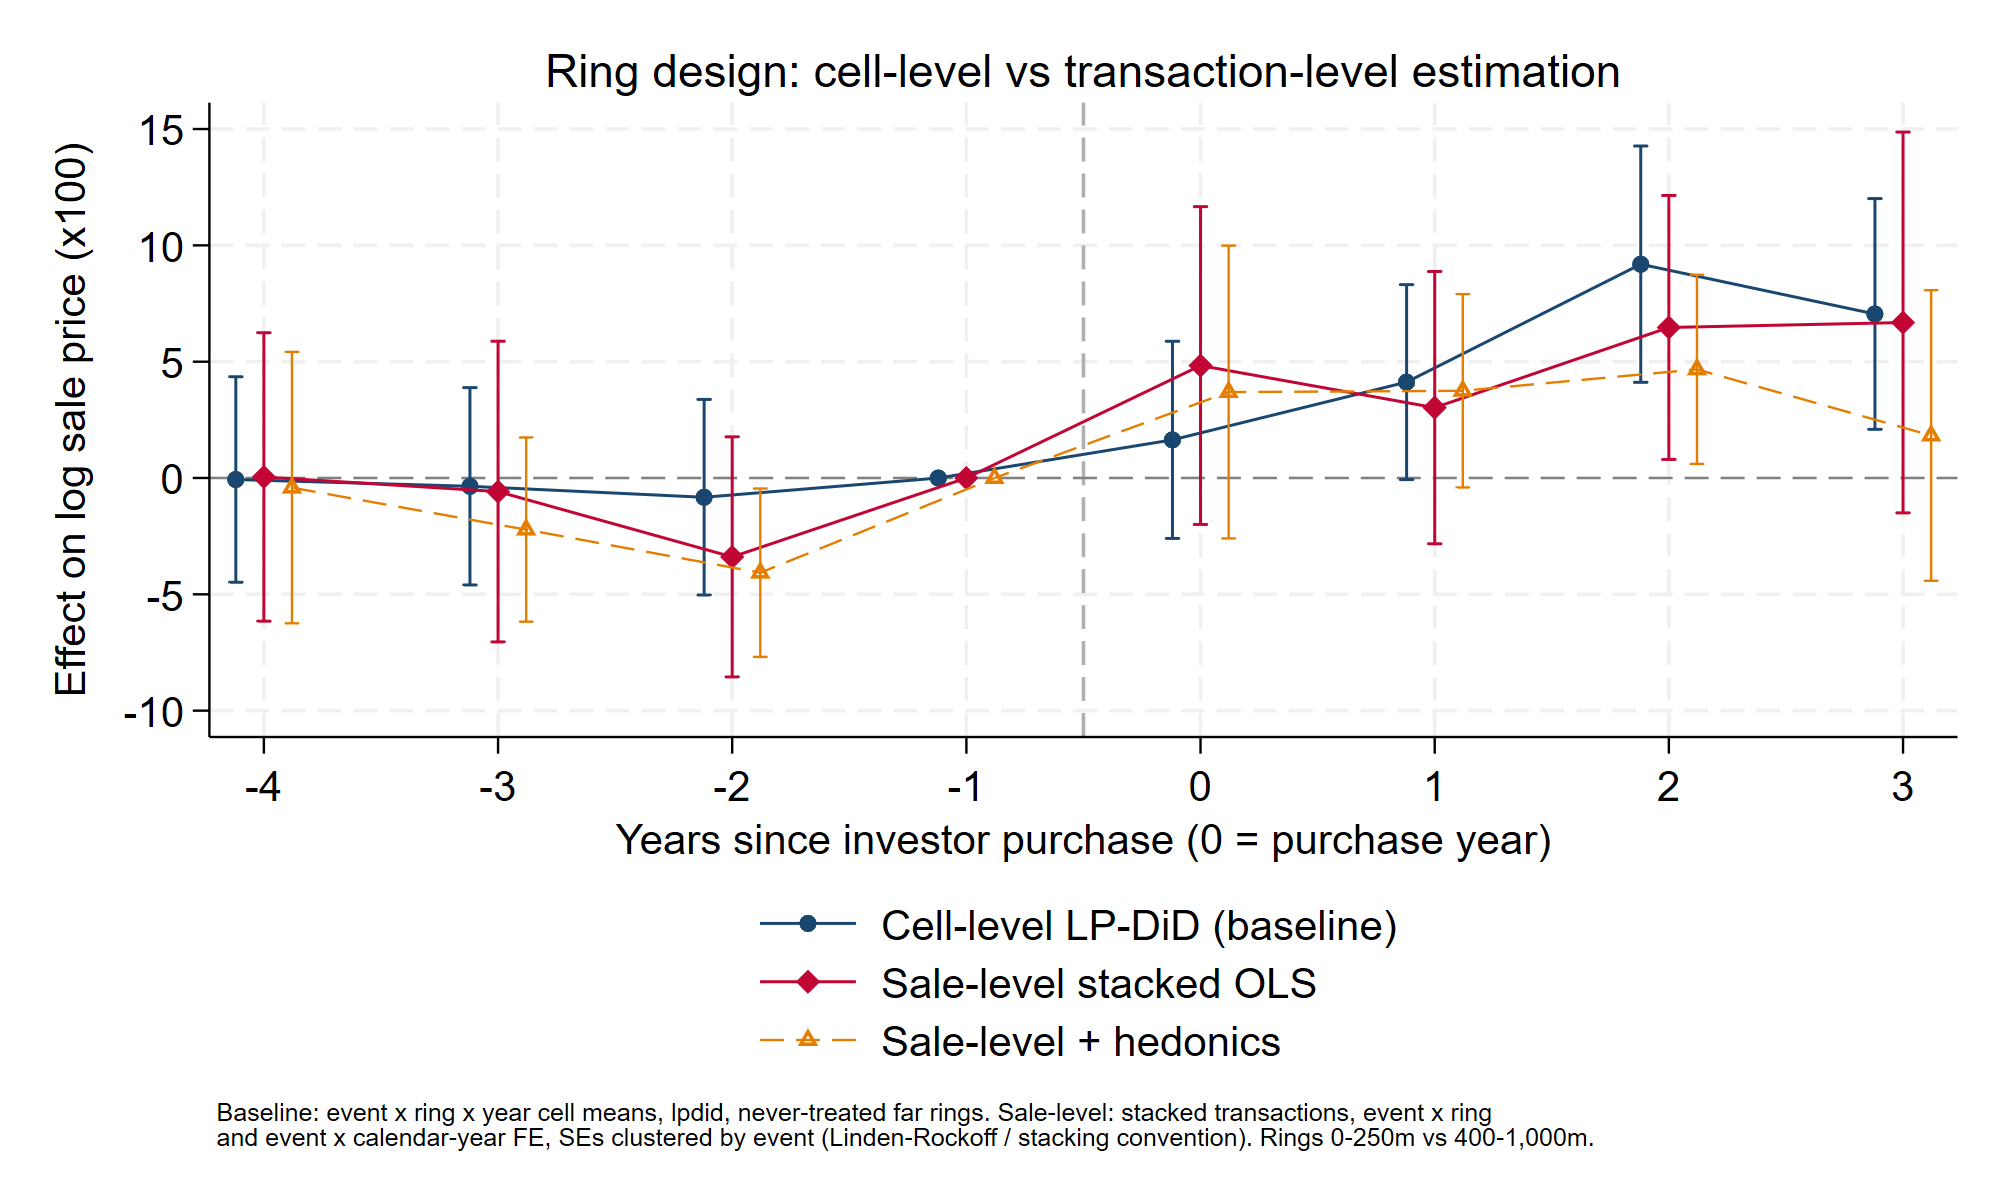
\includegraphics[width=.85\textwidth]{figD12_salelevel_robustness.png}
  \caption{\textbf{Estimation-approach robustness.} The near-ring event study
  estimated three ways: the cell-level LP-DiD baseline; sale-level stacked
  OLS with event$\times$ring and event$\times$calendar-year fixed effects
  (the ring literature's convention), clustered by event; and the sale-level
  specification with hedonic controls. Rings 0--250\,m vs 400--1{,}000\,m.
  The three series coincide within sampling error at every horizon, and the
  agreement of transaction-weighted and event-weighted estimates indicates
  the pooled effect is not driven by a few high-volume events.}
  \label{fig:salelevel}
\end{figure}

In the annual robustness suite $Q = 4$ and $H = 3$; the baseline is also
estimated at quarterly ($Q=H=8$) and half-yearly resolutions and with the
Callaway--Sant'Anna (2021) group-time estimator
$ATT(g,t) = \mathbb{E}[\bar{y}_{t} - \bar{y}_{g-1} \mid G_g = 1] -
\mathbb{E}[\bar{y}_{t} - \bar{y}_{g-1} \mid \text{never treated}]$,
aggregated to event time; results are similar across estimators and
resolutions, and identical with and without tract fixed effects.

\section{The eight figures}

All figures plot LP-DiD event-study coefficients
$\{\beta_{-Q},\dots,\beta_{H}\}$ from
equations~\eqref{eq:lpdid_post}--\eqref{eq:lpdid_pre} at annual resolution
(pre-window 4, post-window 3), with 95\% confidence intervals, cells clustered.
Period $-1$ is the omitted base; the dashed vertical line marks the treatment
boundary.

\begin{figure}[htbp]
  \centering
  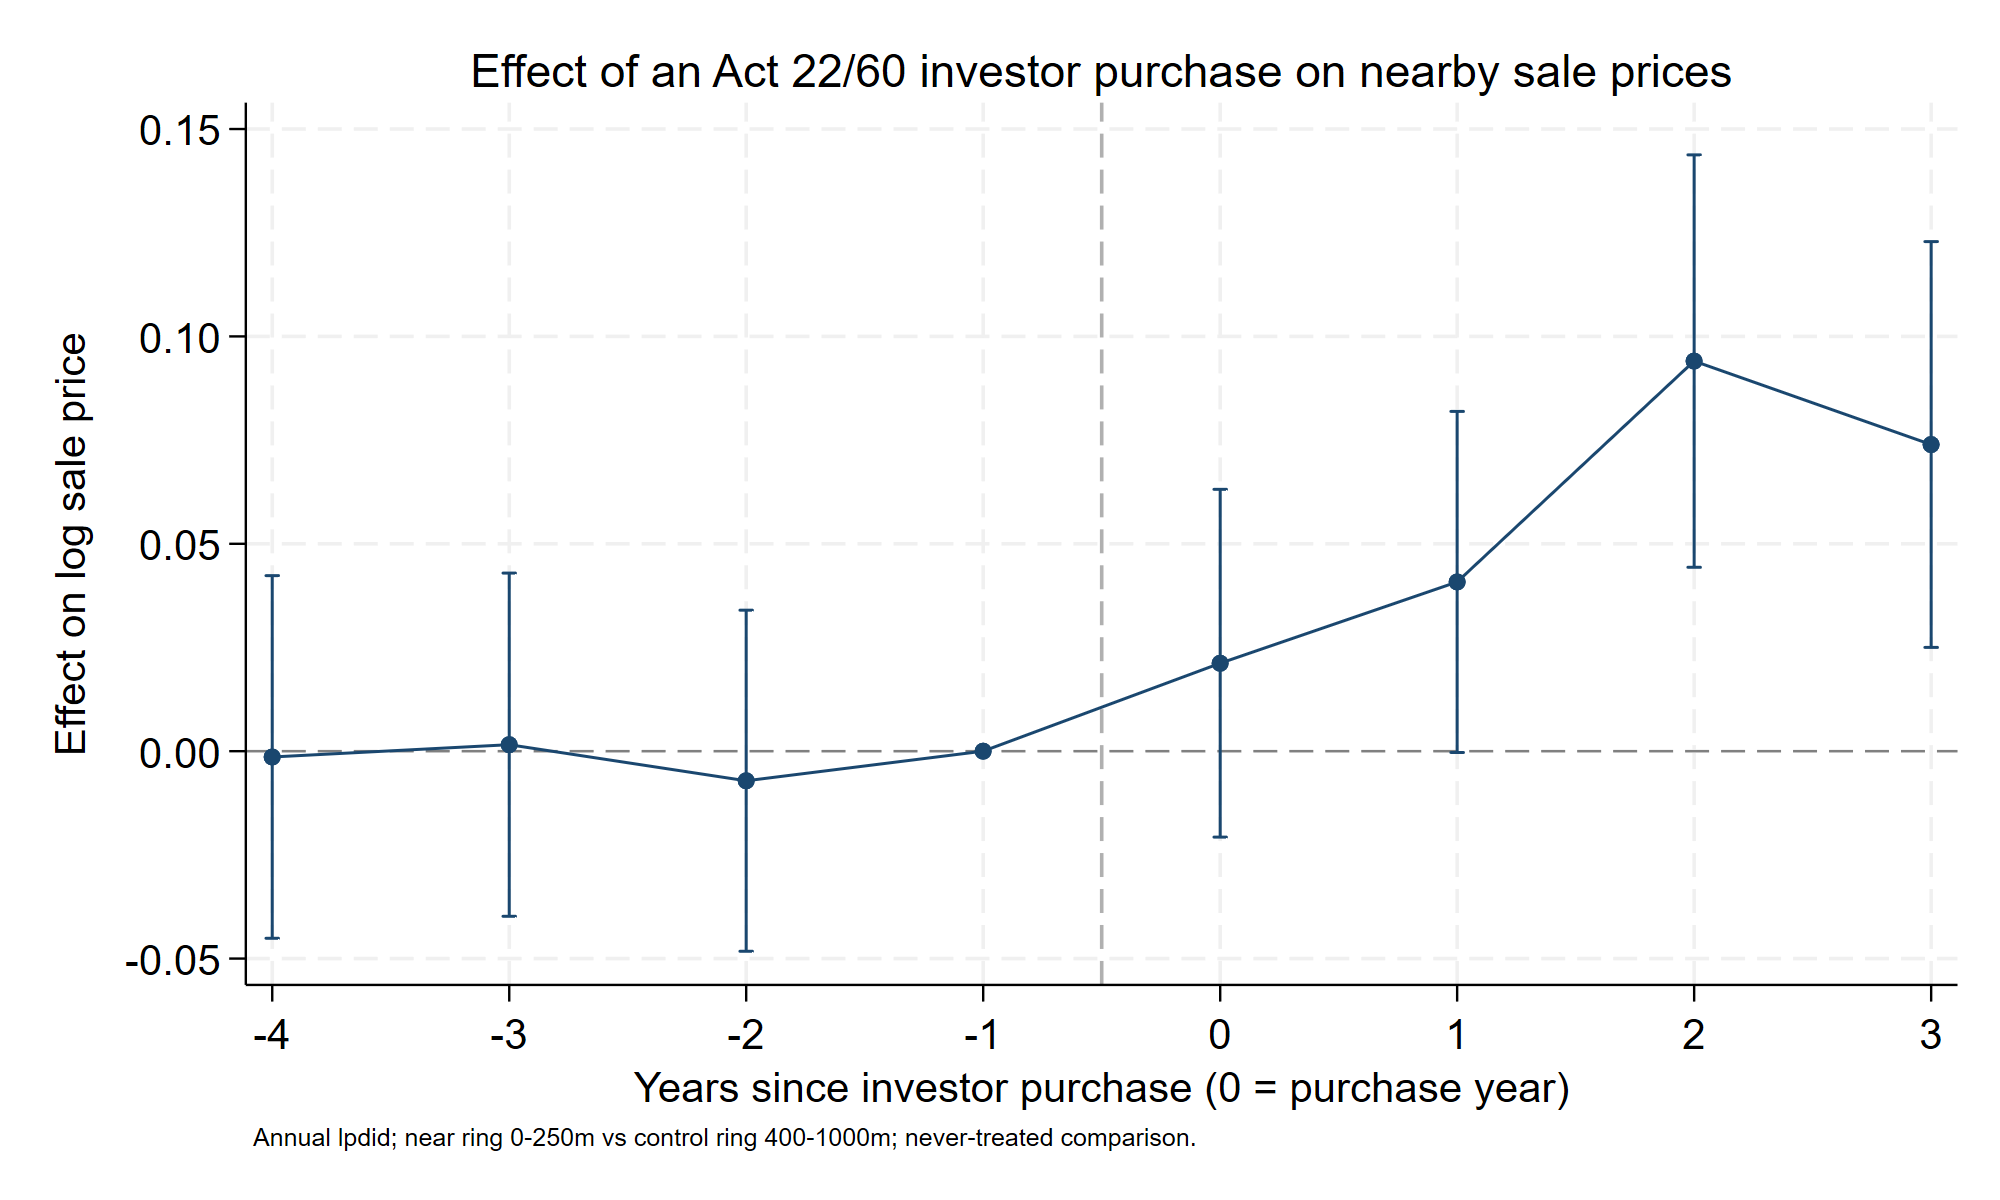
\includegraphics[width=.85\textwidth]{fig1_baseline.png}
  \caption{\textbf{Baseline event study.} Near-ring (0--250\,m) versus
  far-ring (400--1{,}000\,m) effects on log sale price by year relative to the
  investor purchase. The headline price bump; flat pre-period coefficients are
  the design's core credibility check, and the post-period path shows how
  quickly the premium appears and whether it persists.}
  \label{fig:baseline}
\end{figure}

\begin{figure}[htbp]
  \centering
  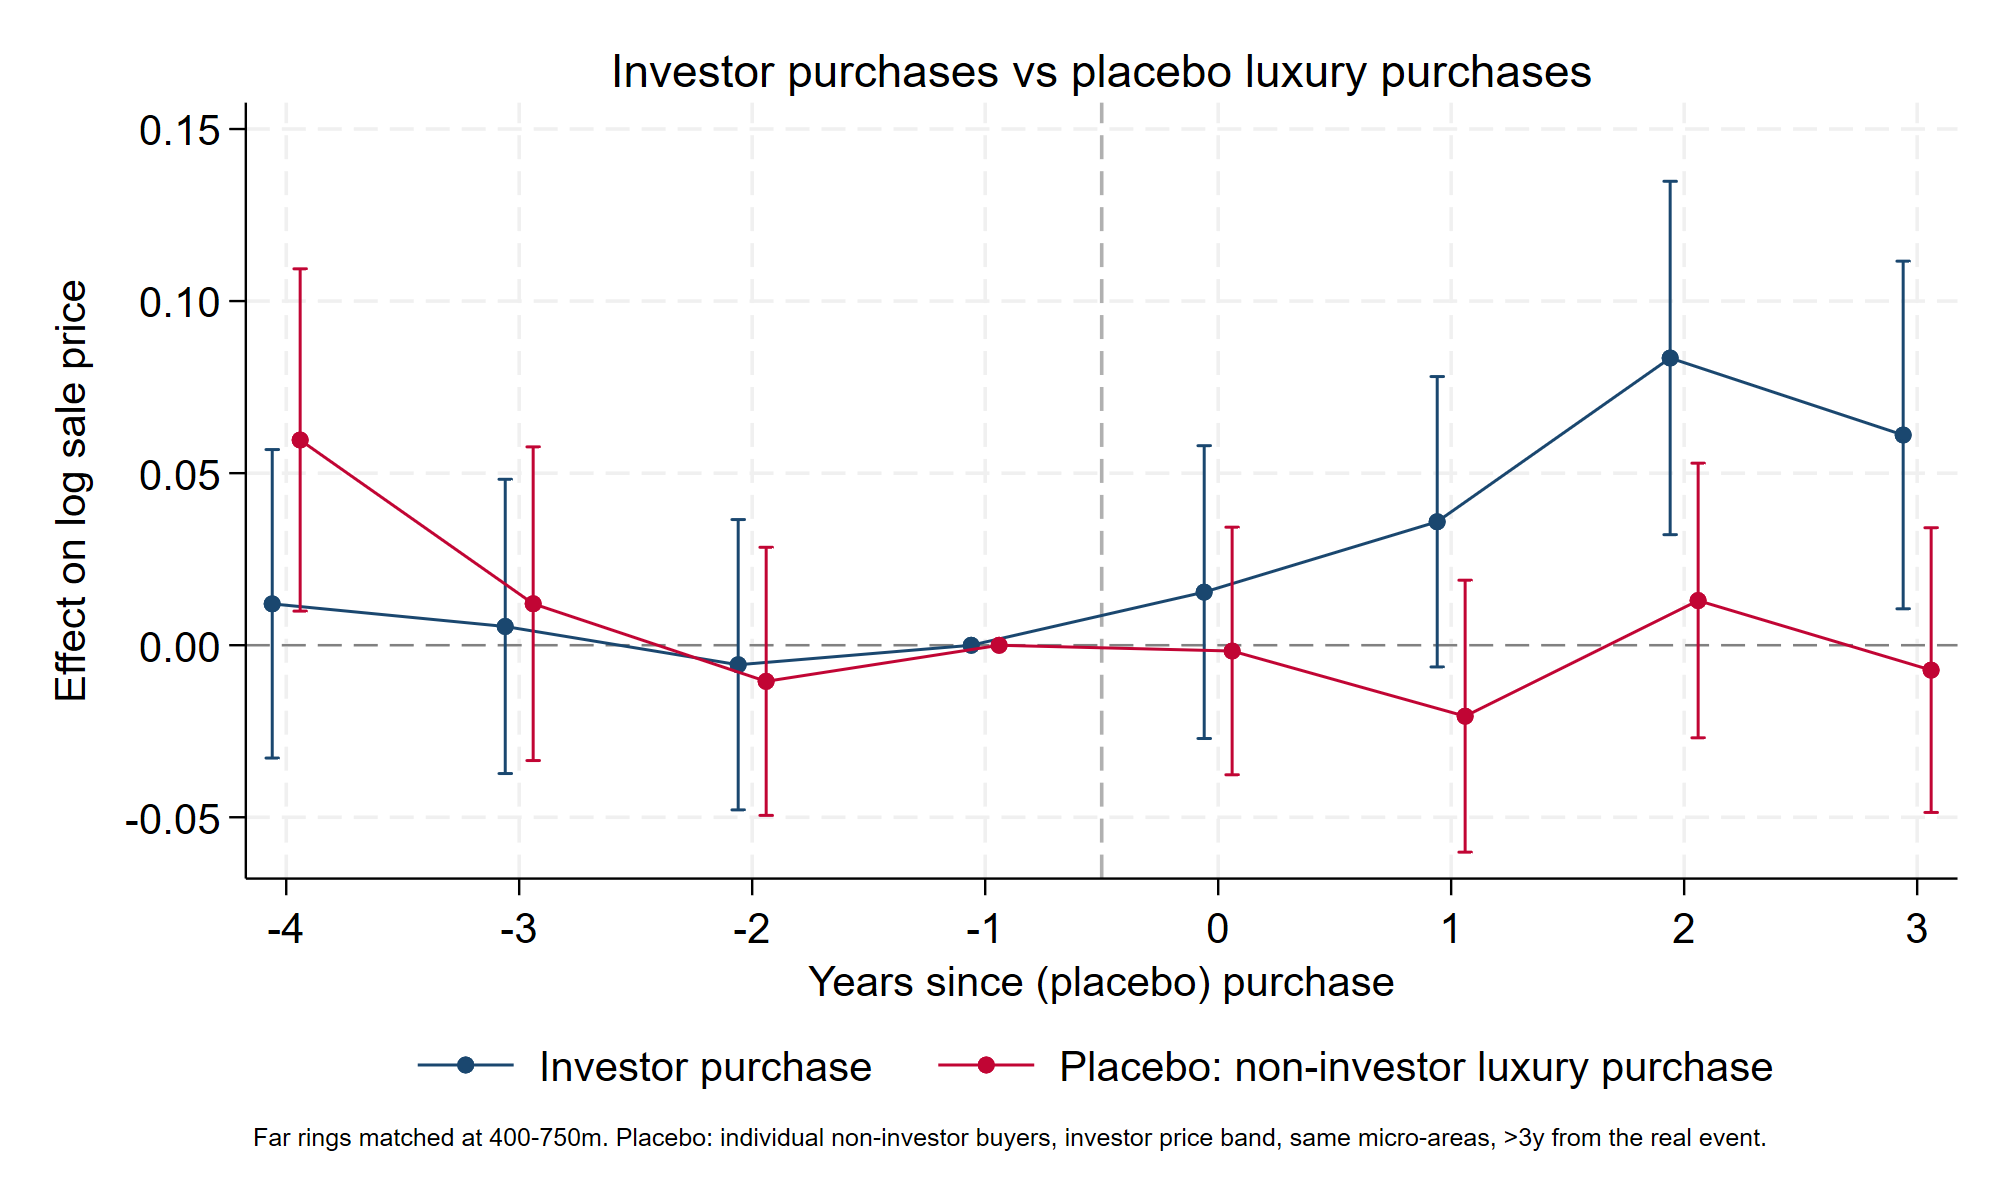
\includegraphics[width=.85\textwidth]{fig2_real_vs_placebo.png}
  \caption{\textbf{Investor vs.\ placebo purchases.} The real event study
  overlaid with placebo events (non-investor individual buyers in the investor
  price band, same micro-areas, $>$3 years from the real event; far rings
  matched at 400--750\,m). A flat placebo says nearby prices respond to
  \emph{the investor}, not to any high-value transaction; because unmatched
  investors contaminate the placebo toward finding an effect, a null placebo
  is conservative evidence of investor specificity.}
  \label{fig:placebo}
\end{figure}

\begin{figure}[htbp]
  \centering
  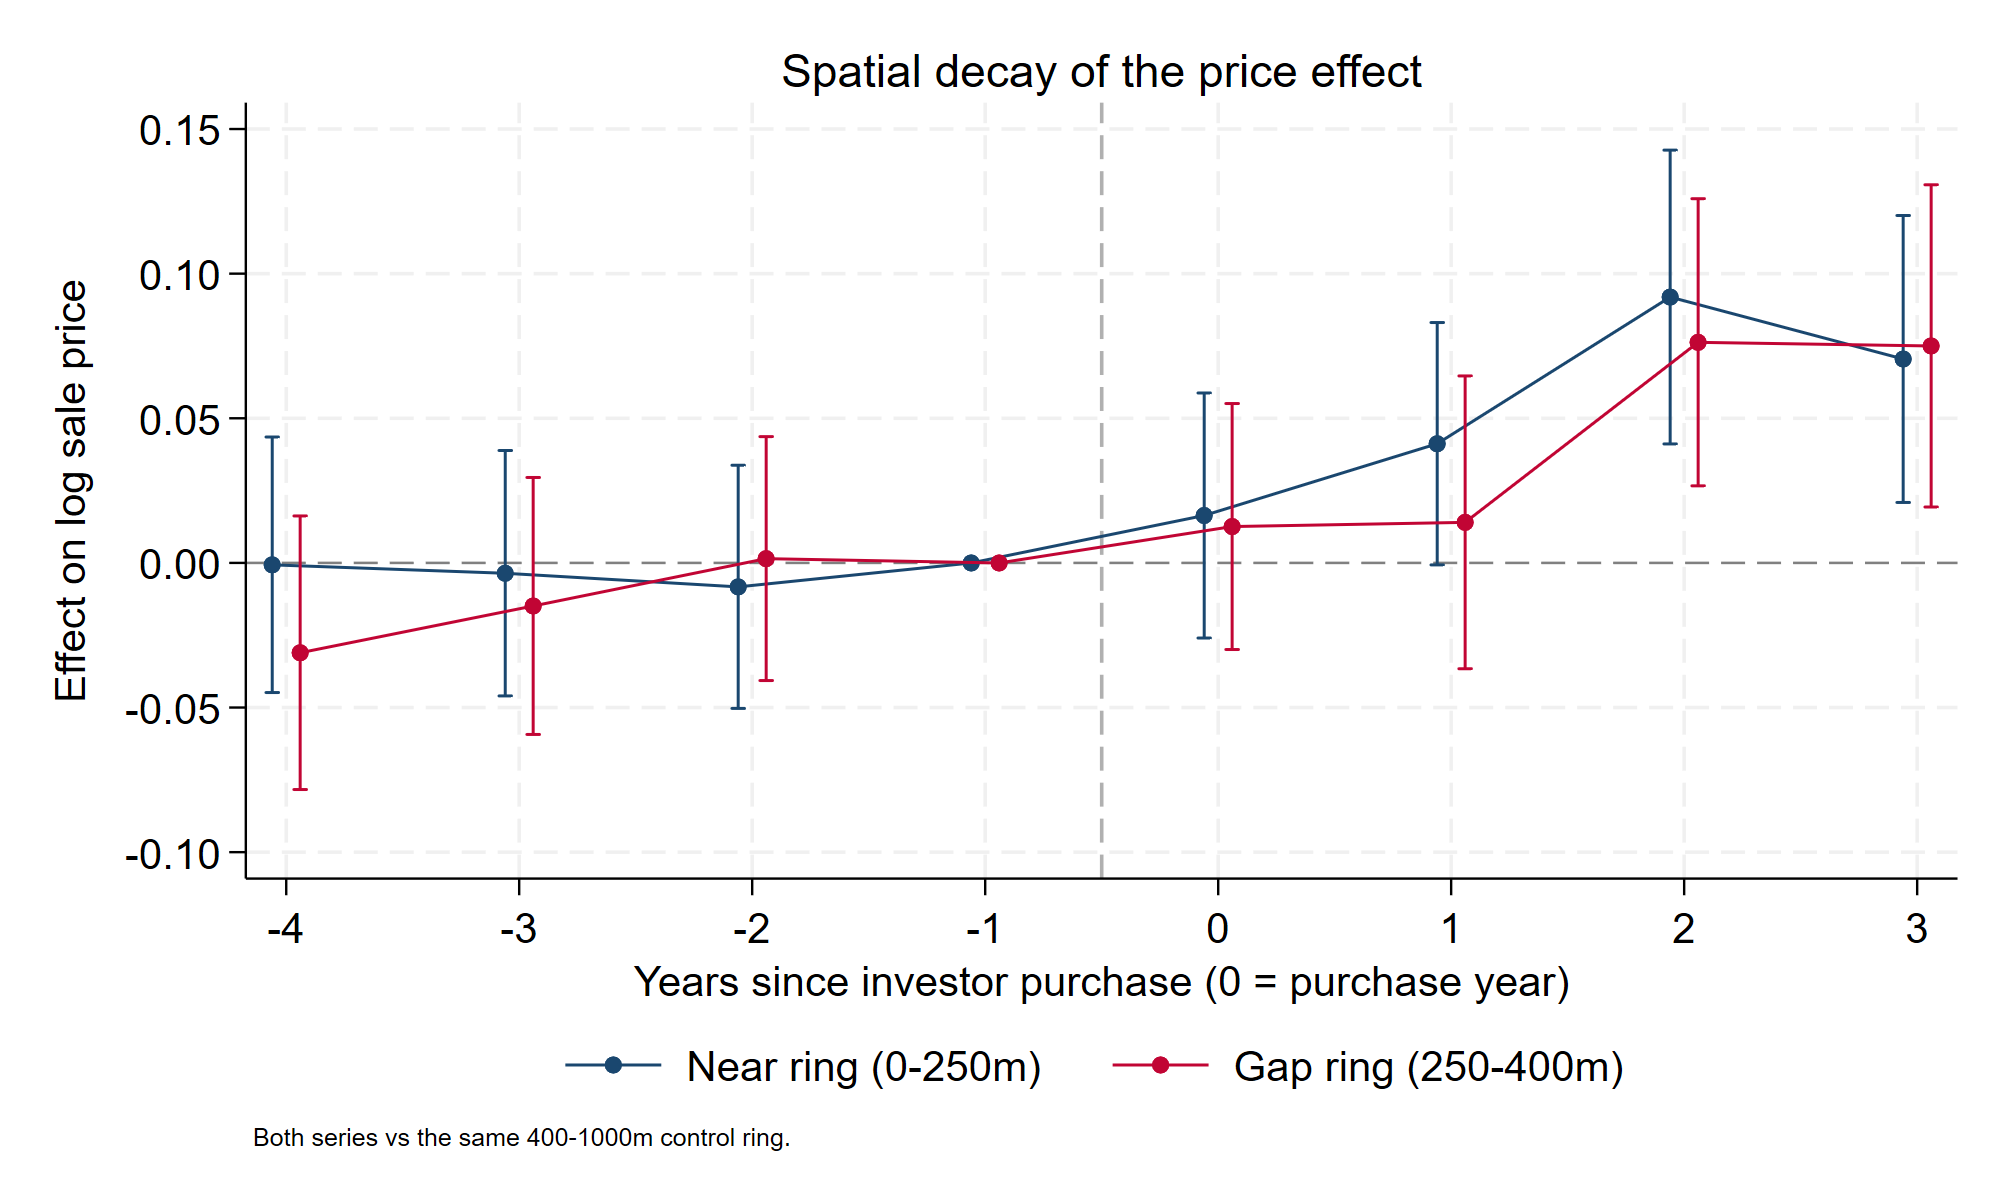
\includegraphics[width=.85\textwidth]{fig3_gradient.png}
  \caption{\textbf{Spatial gradient.} Near-ring (0--250\,m) and gap-ring
  (250--400\,m) series, each against the same far control. A genuine
  hyper-local spillover should decay with distance
  ($\text{near} > \text{gap} > 0$); near $\approx$ gap would instead indicate
  a neighborhood-wide shock partially shared by the control ring.}
  \label{fig:gradient}
\end{figure}

\begin{figure}[htbp]
  \centering
  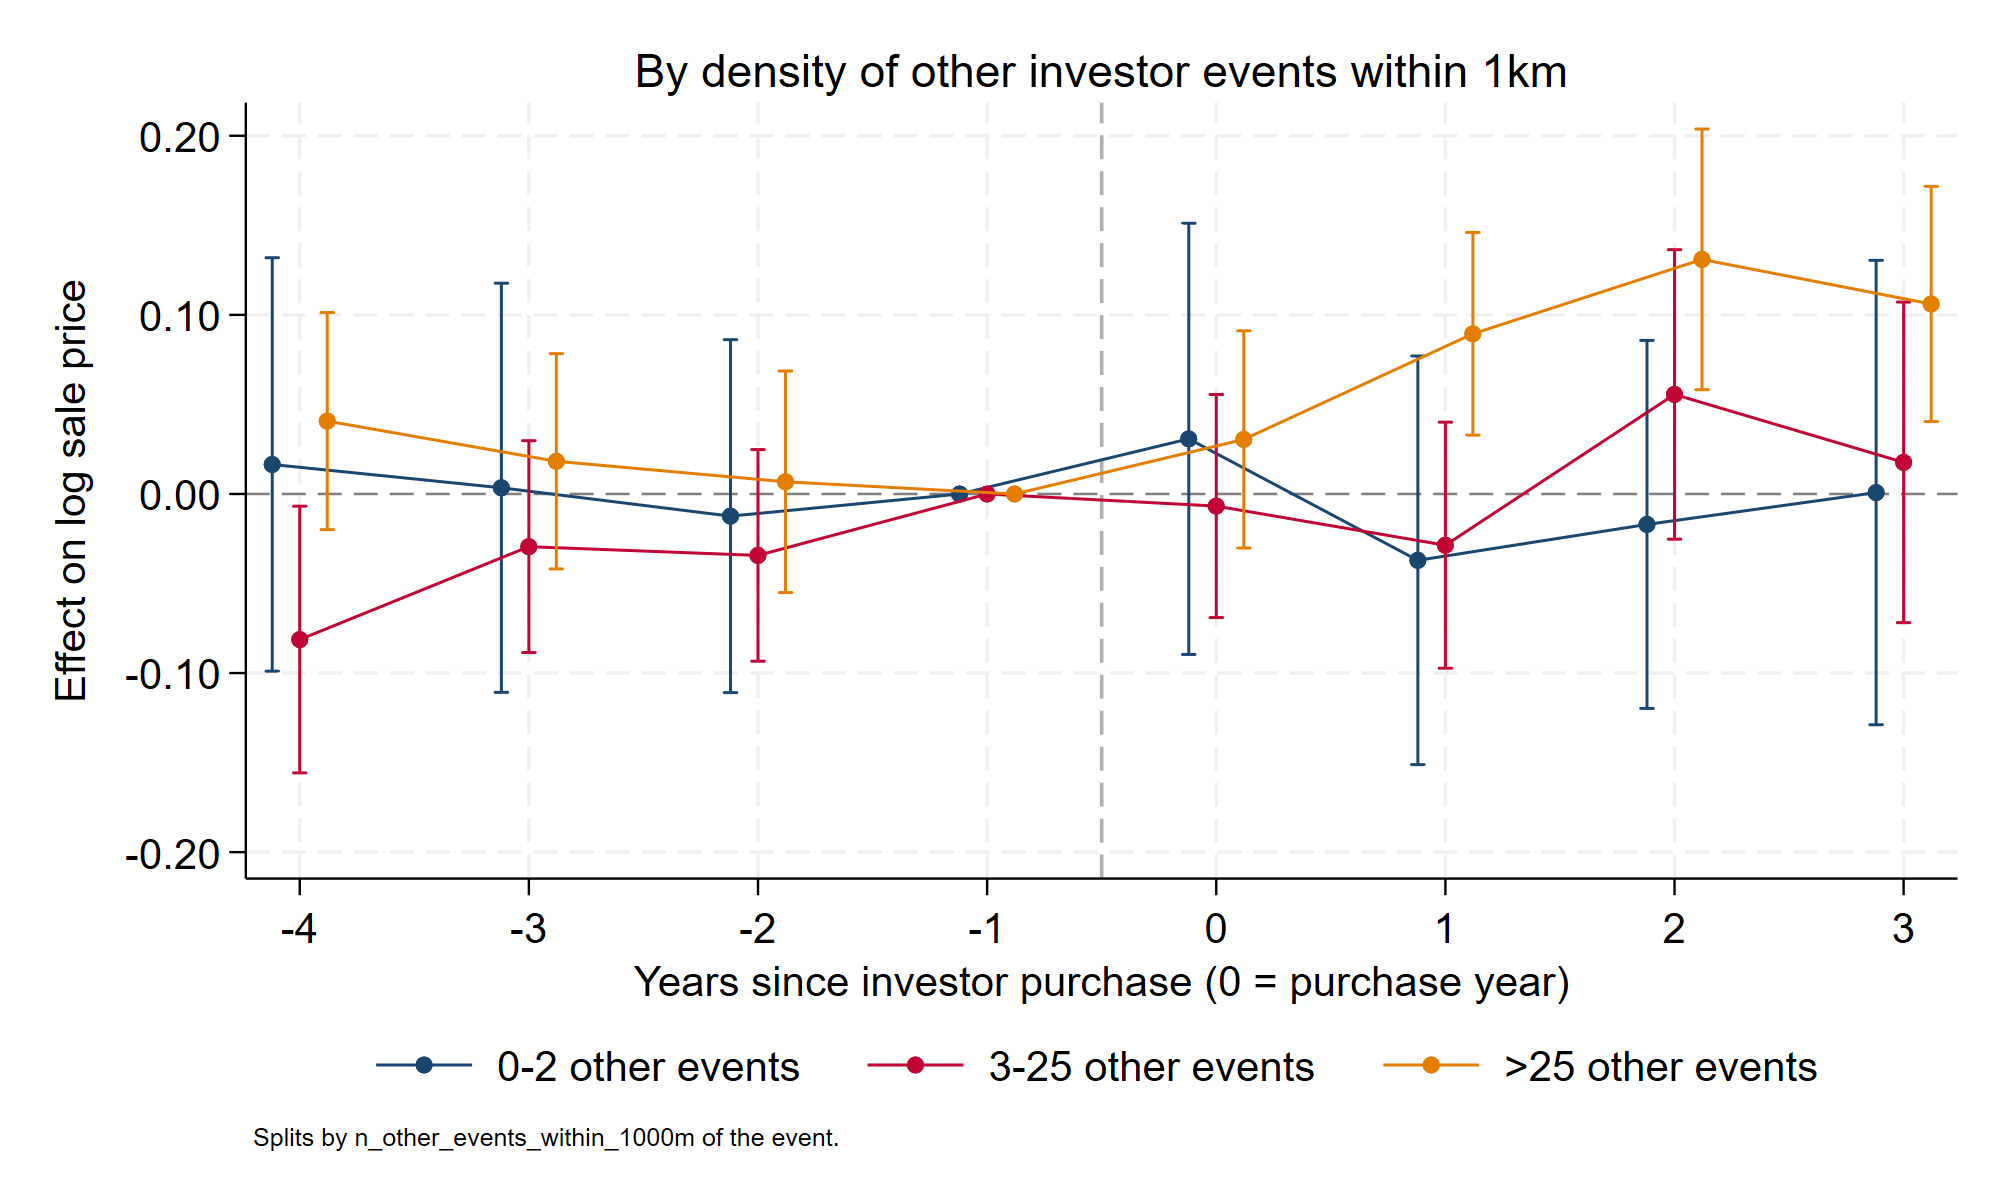
\includegraphics[width=.85\textwidth]{fig4_dose.png}
  \caption{\textbf{Estimated contrast by local event density.} Separate event
  studies for events with 0--2, 3--25, and $>$25 other investor events within
  1\,km. Because purchases cluster at the enclave scale (condo buildings,
  resort communities), other events in dense areas fall disproportionately
  \emph{inside} the near ring, so the near--far contrast there reflects
  cumulative local investor exposure rather than a single purchase. The
  estimated effect is increasing in density and near zero for isolated
  events: single-purchase channels (comps entry, one renovation, signaling)
  appear weak on their own, and the price response is a phenomenon of investor
  \emph{concentration}. Pre-period coefficients are flat in all
  three density groups, inconsistent with investor waves selecting into
  already-appreciating pockets.}
  \label{fig:dose}
\end{figure}

\begin{figure}[htbp]
  \centering
  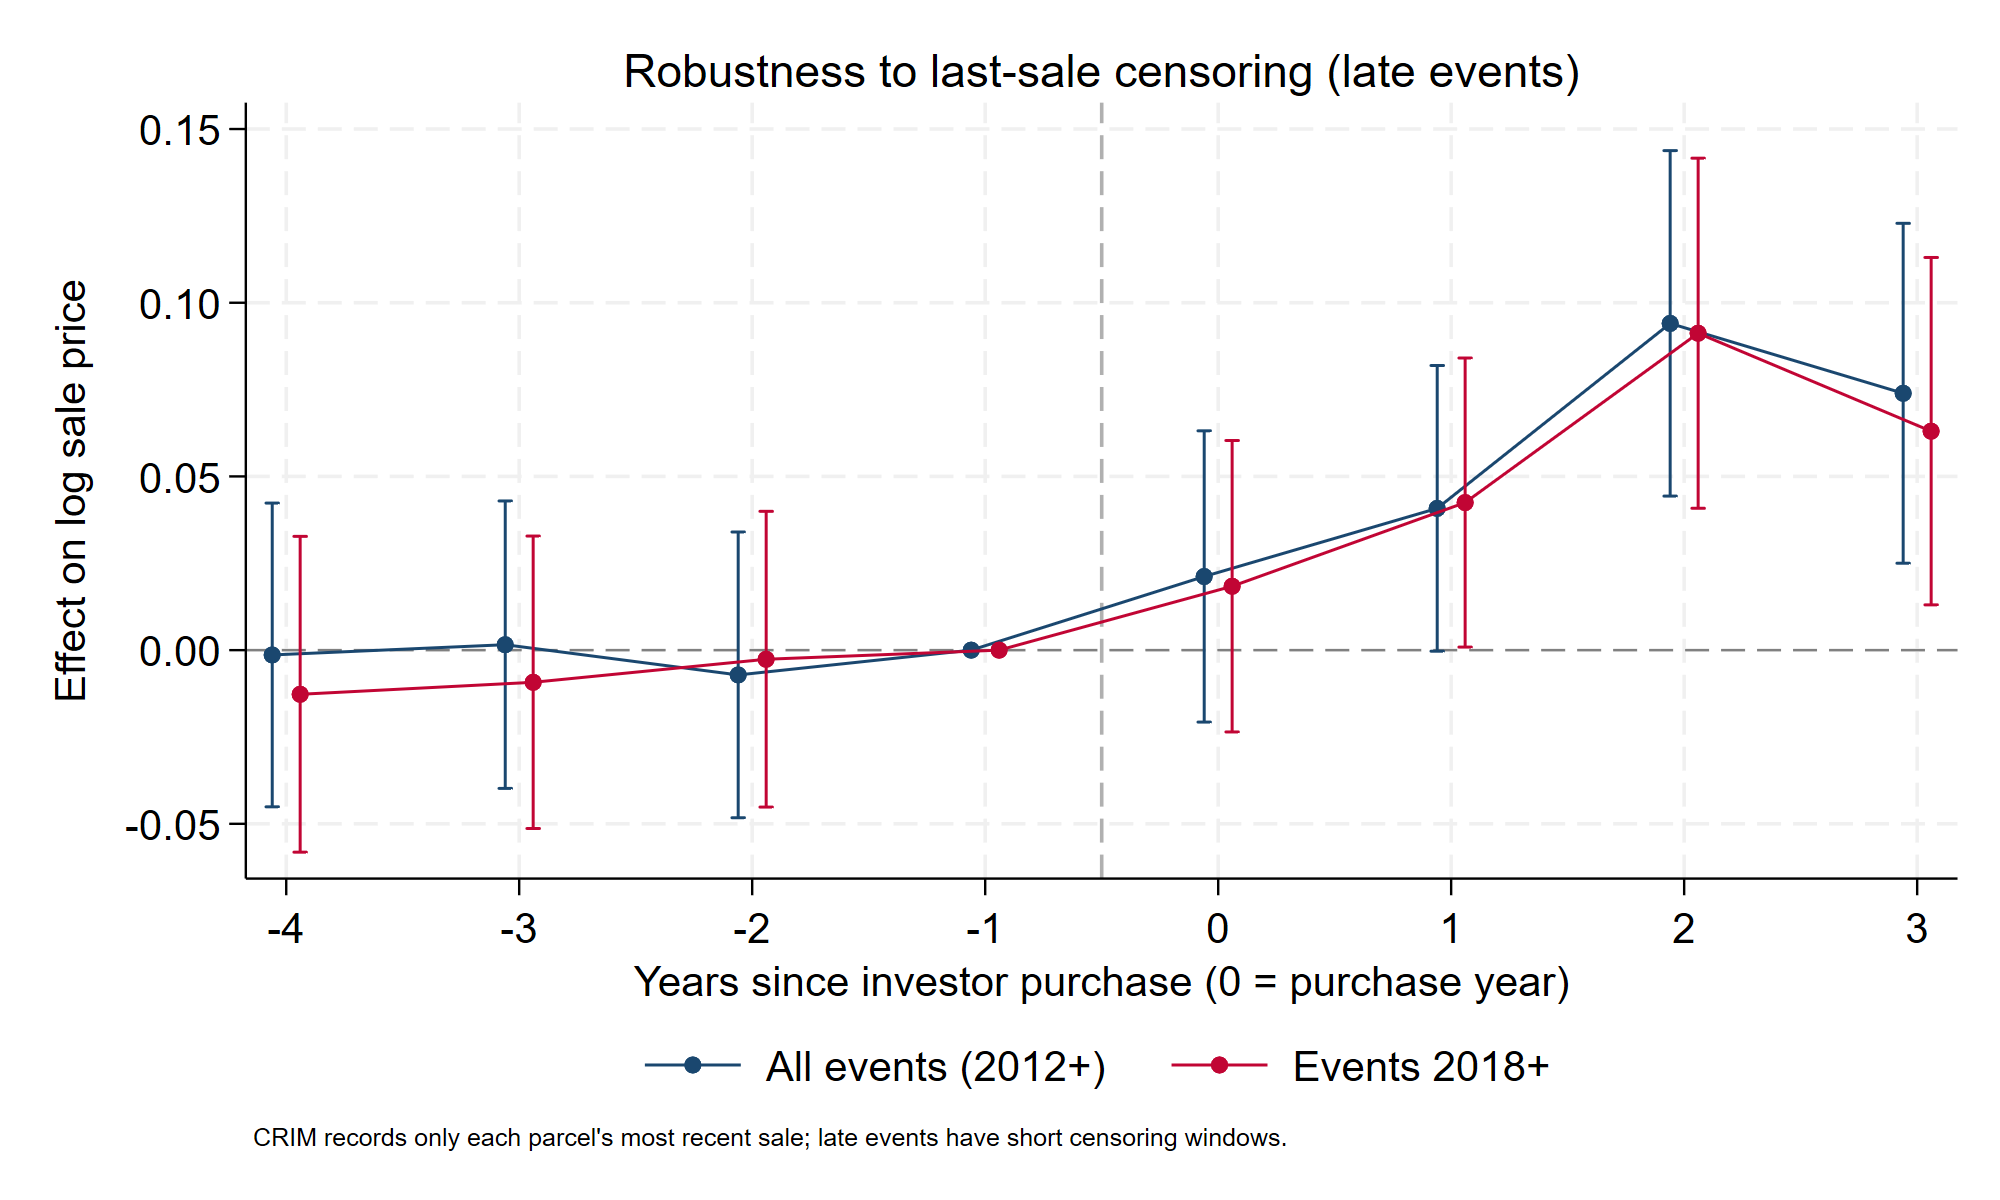
\includegraphics[width=.85\textwidth]{fig5_late.png}
  \caption{\textbf{Censoring robustness.} Baseline overlaid with events from
  2018 onward, for which little time exists for post-period sales to be
  overwritten by later resales. Agreement with the full sample indicates that
  CRIM's last-sale-only censoring is not manufacturing the bump.}
  \label{fig:late}
\end{figure}

\begin{figure}[htbp]
  \centering
  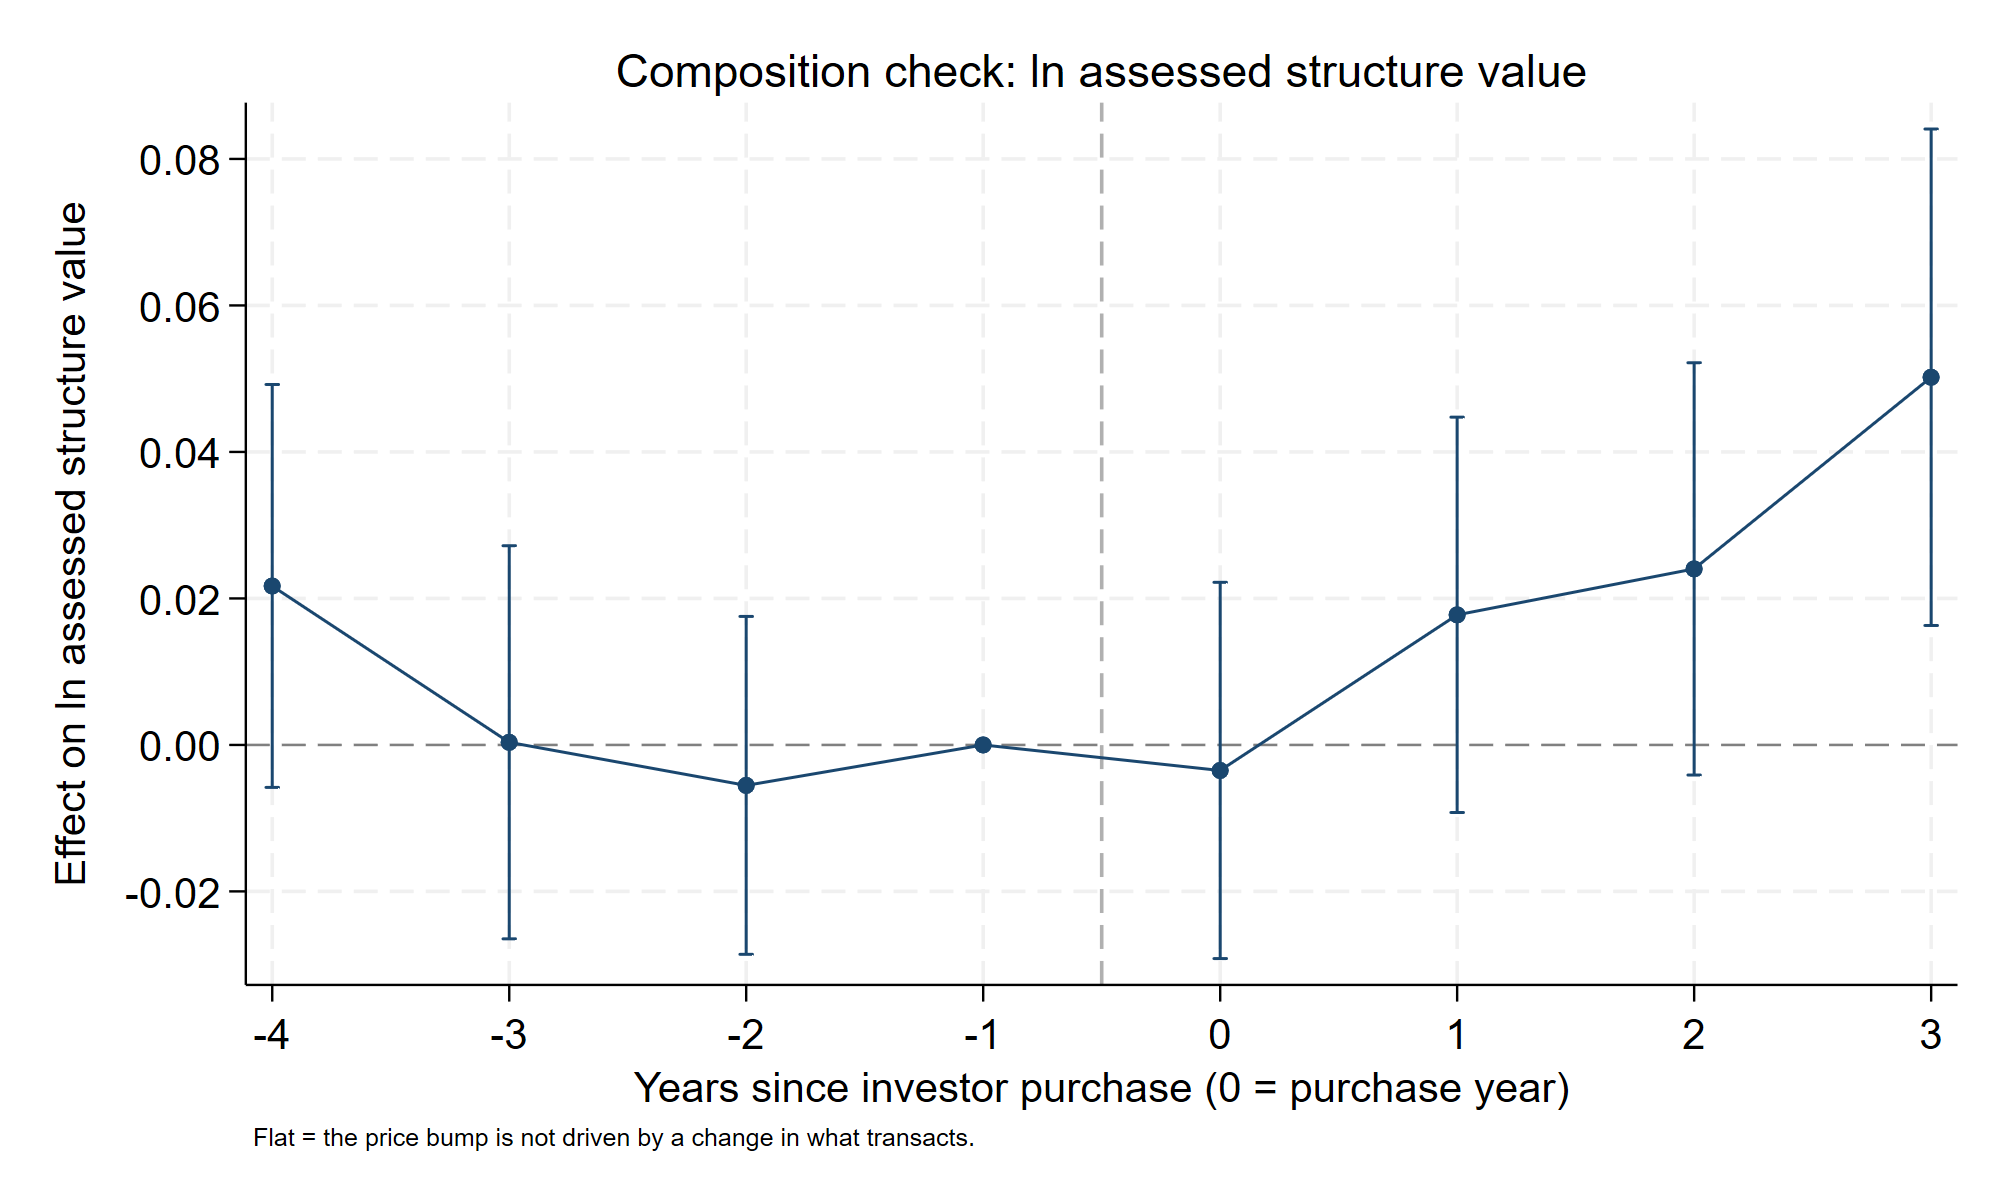
\includegraphics[width=.48\textwidth]{fig6_comp_lnstru.png}\hfill
  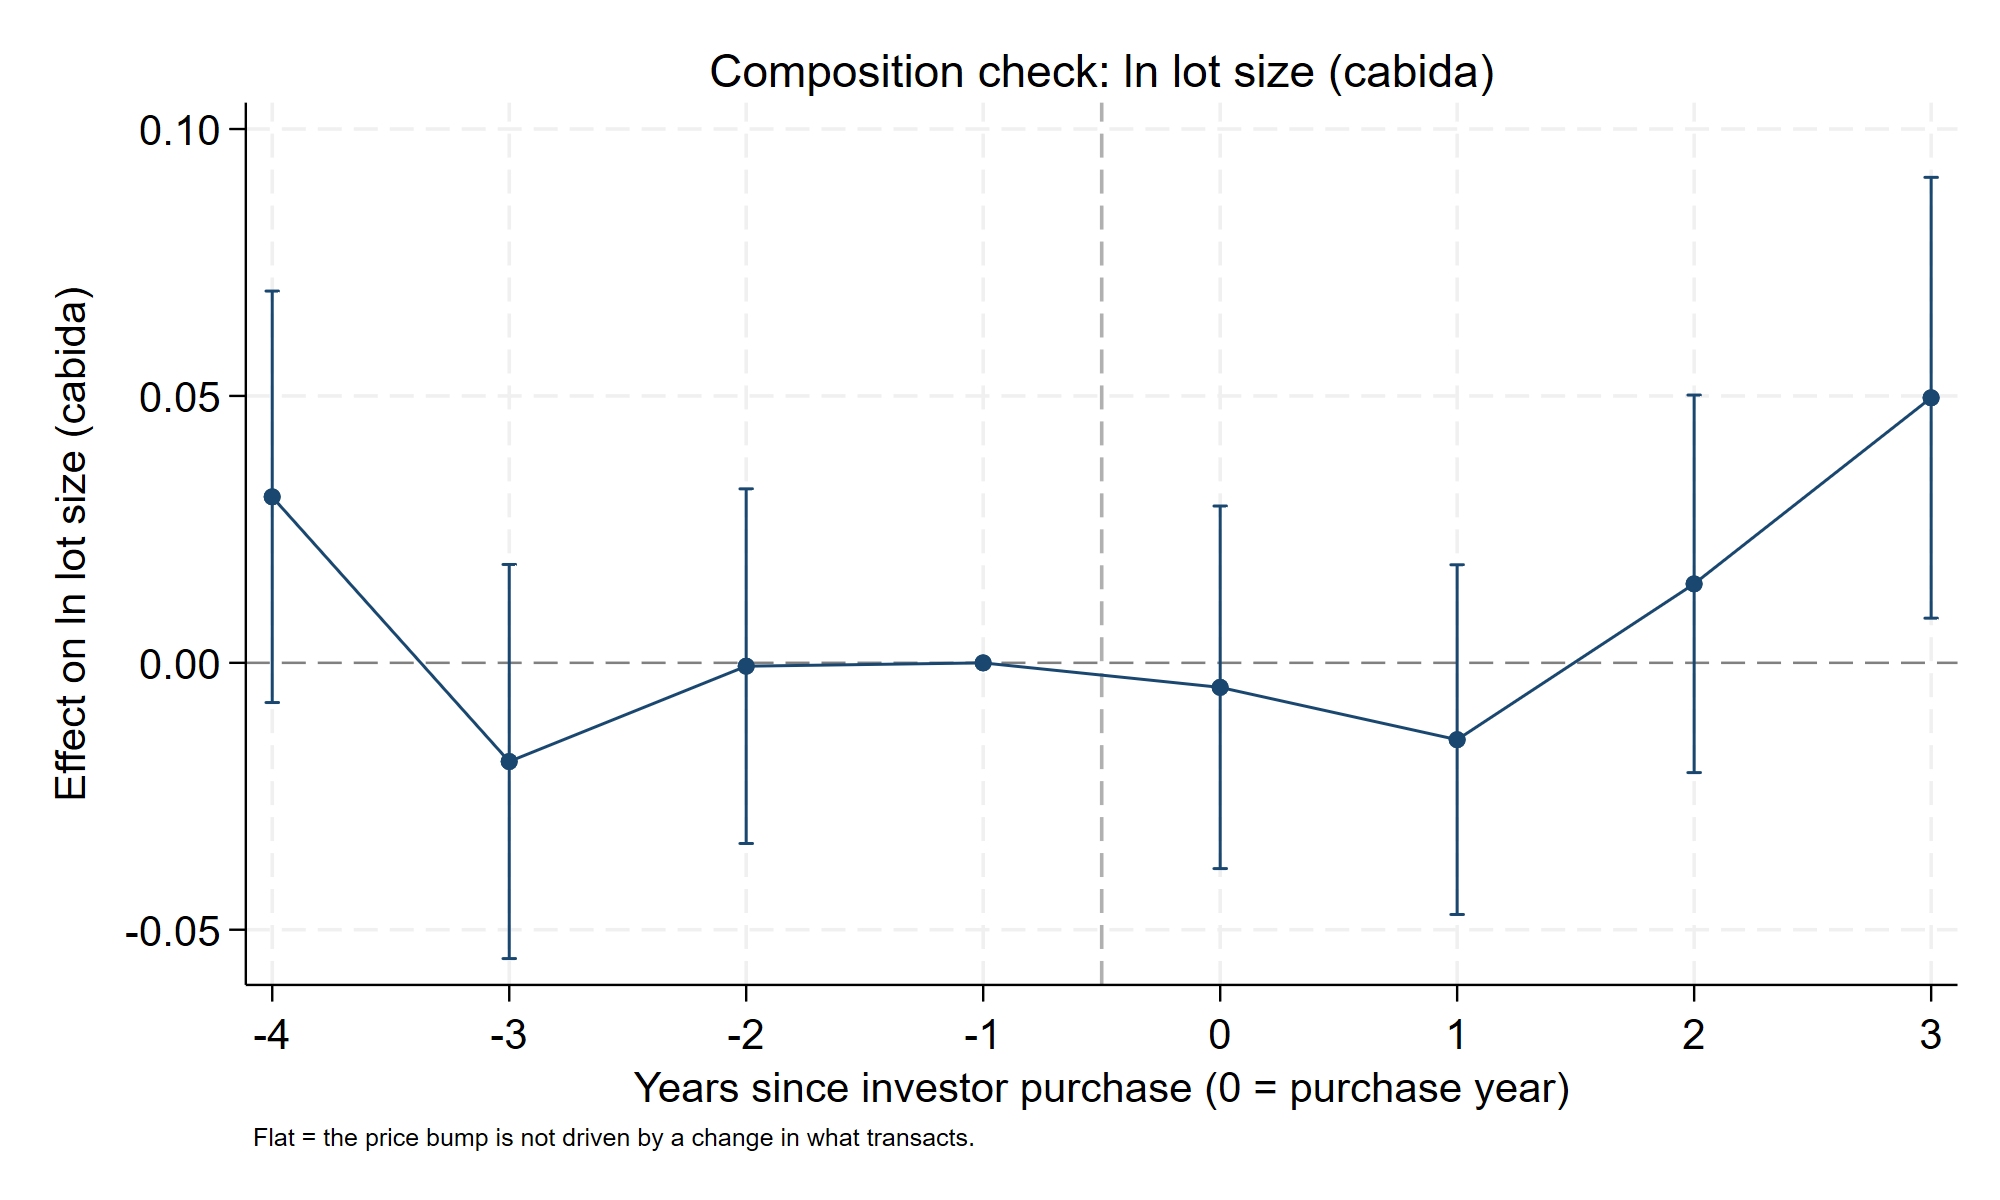
\includegraphics[width=.48\textwidth]{fig6_comp_lncab.png}\\[2pt]
  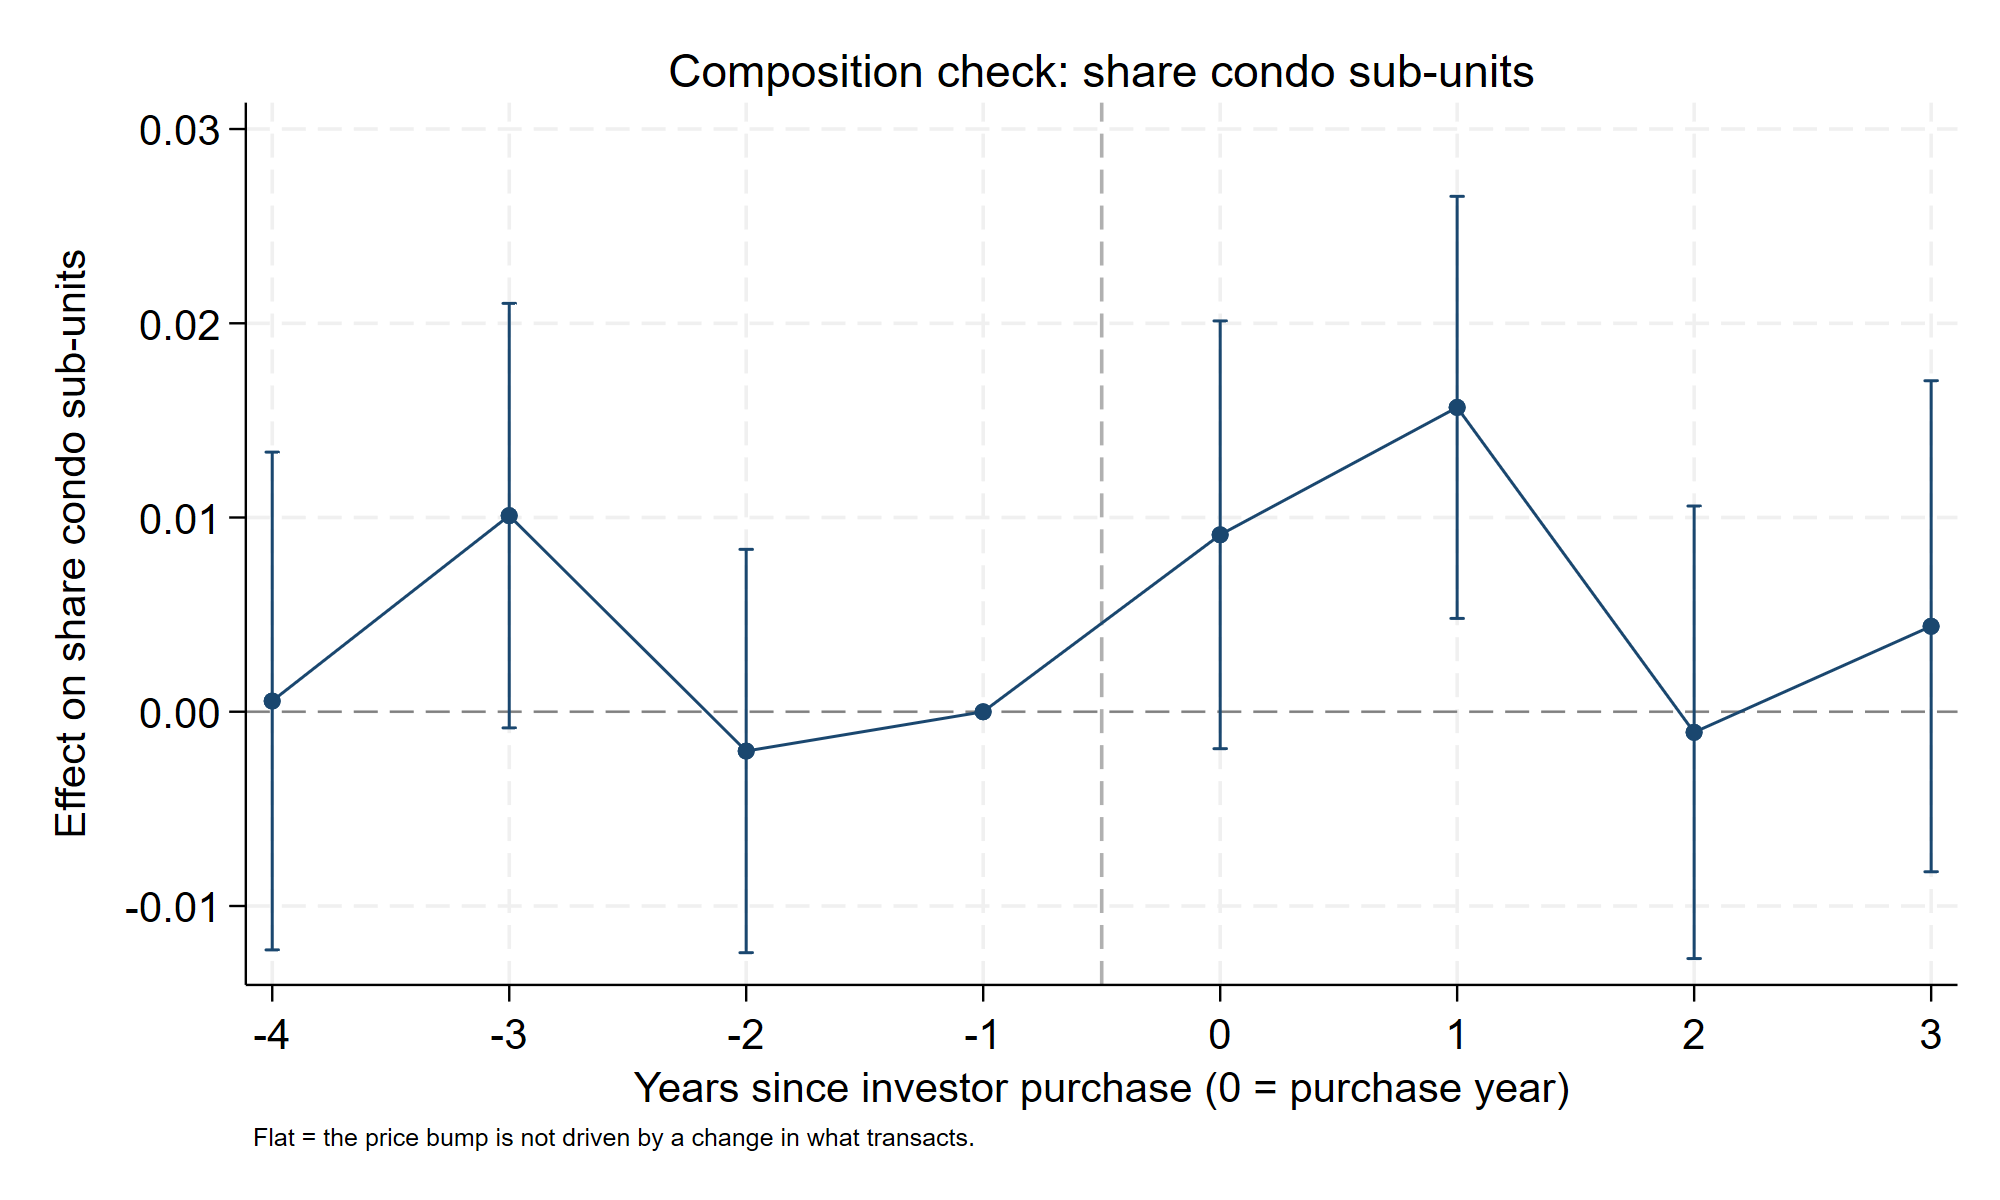
\includegraphics[width=.48\textwidth]{fig6_comp_subu.png}\hfill
  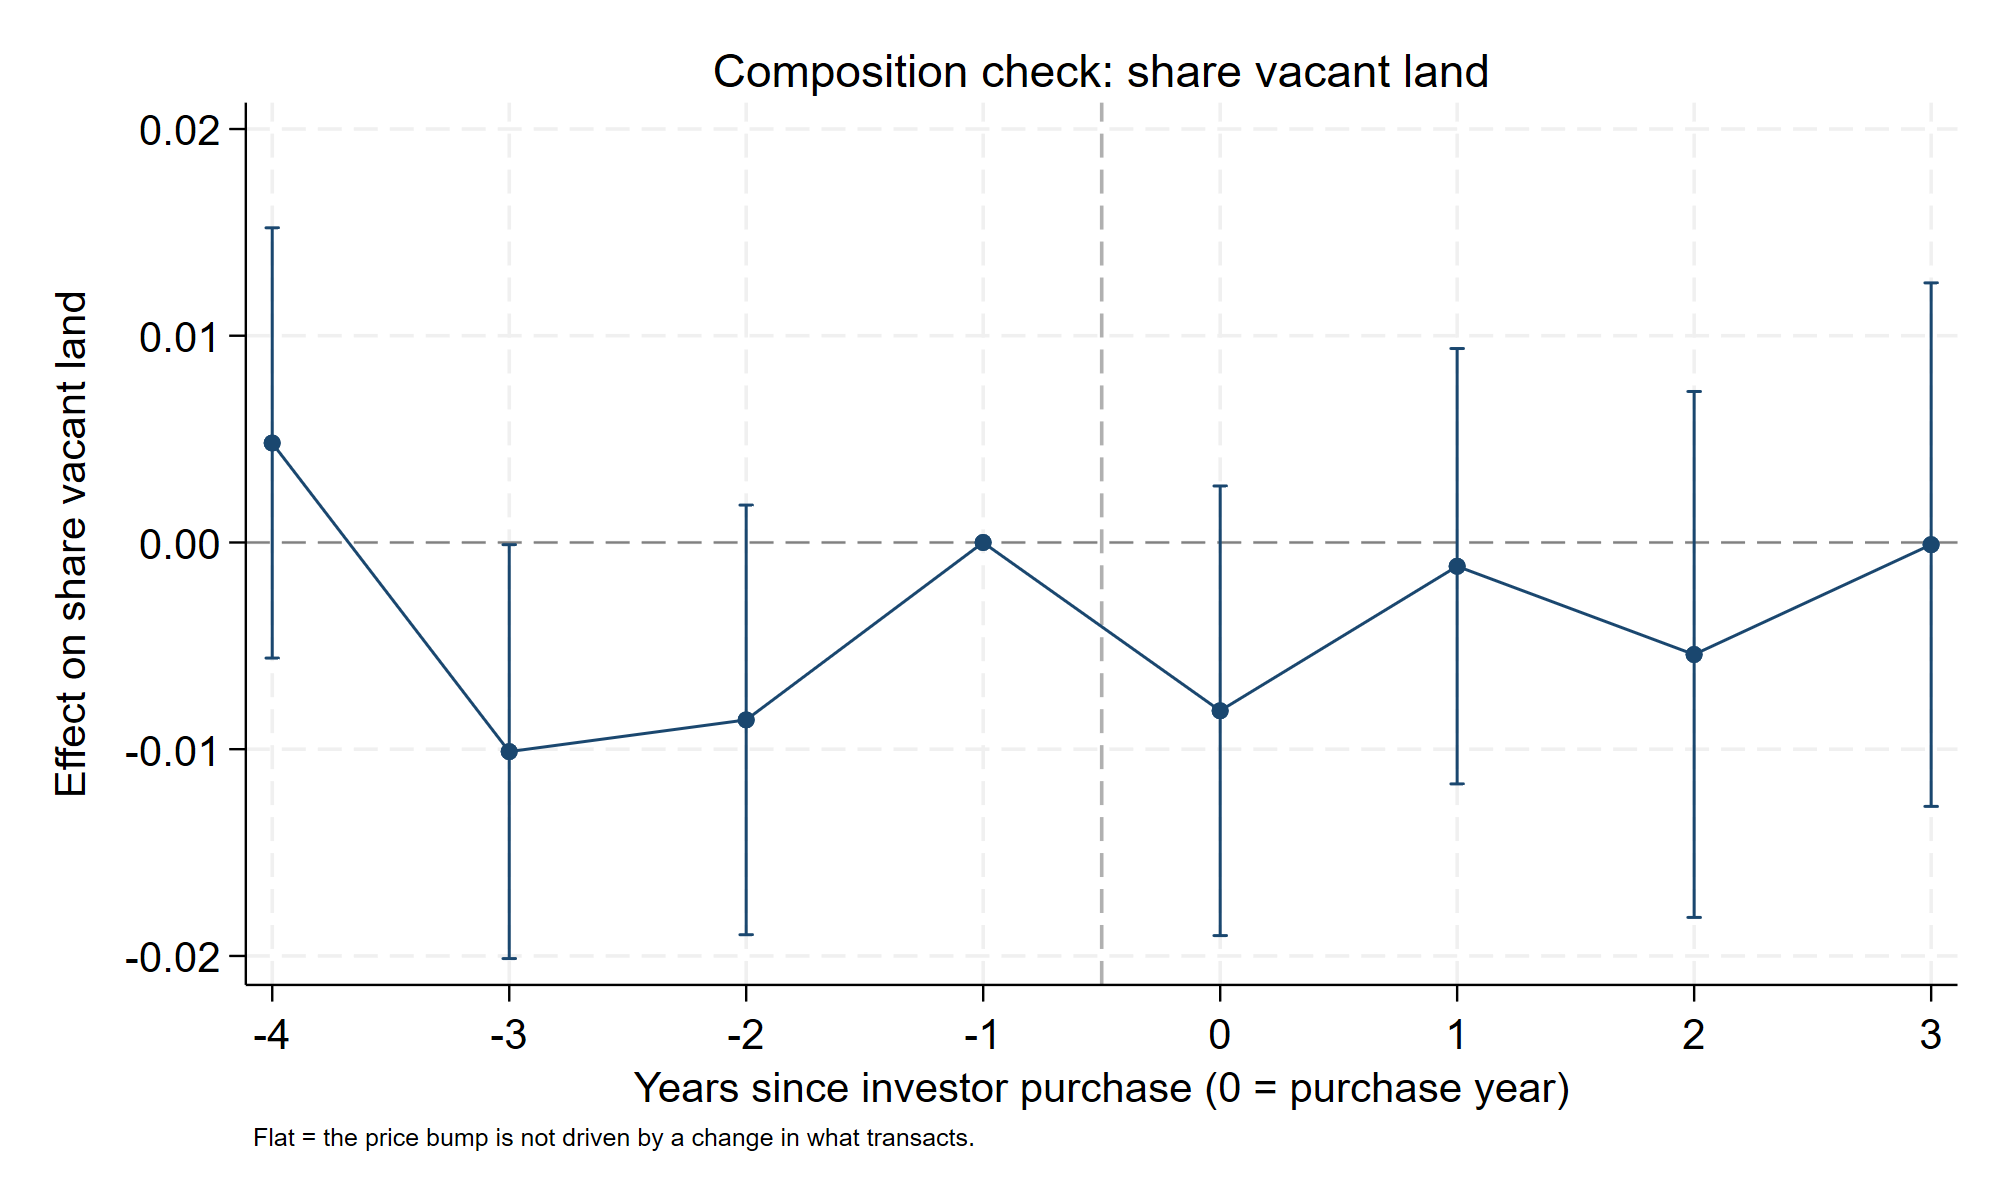
\includegraphics[width=.48\textwidth]{fig6_comp_vac.png}
  \caption{\textbf{Composition checks.} The identical design with property
  characteristics as outcomes: log assessed structure value (top left), log
  lot size (top right), condo-unit share (bottom left), vacant-land share
  (bottom right). Flat lines imply the price bump is appreciation on a stable
  transaction mix; movements would reveal the stock-upgrading margin of
  gentrification, changing the interpretation of Figure~\ref{fig:baseline}.}
  \label{fig:composition}
\end{figure}

\begin{figure}[htbp]
  \centering
  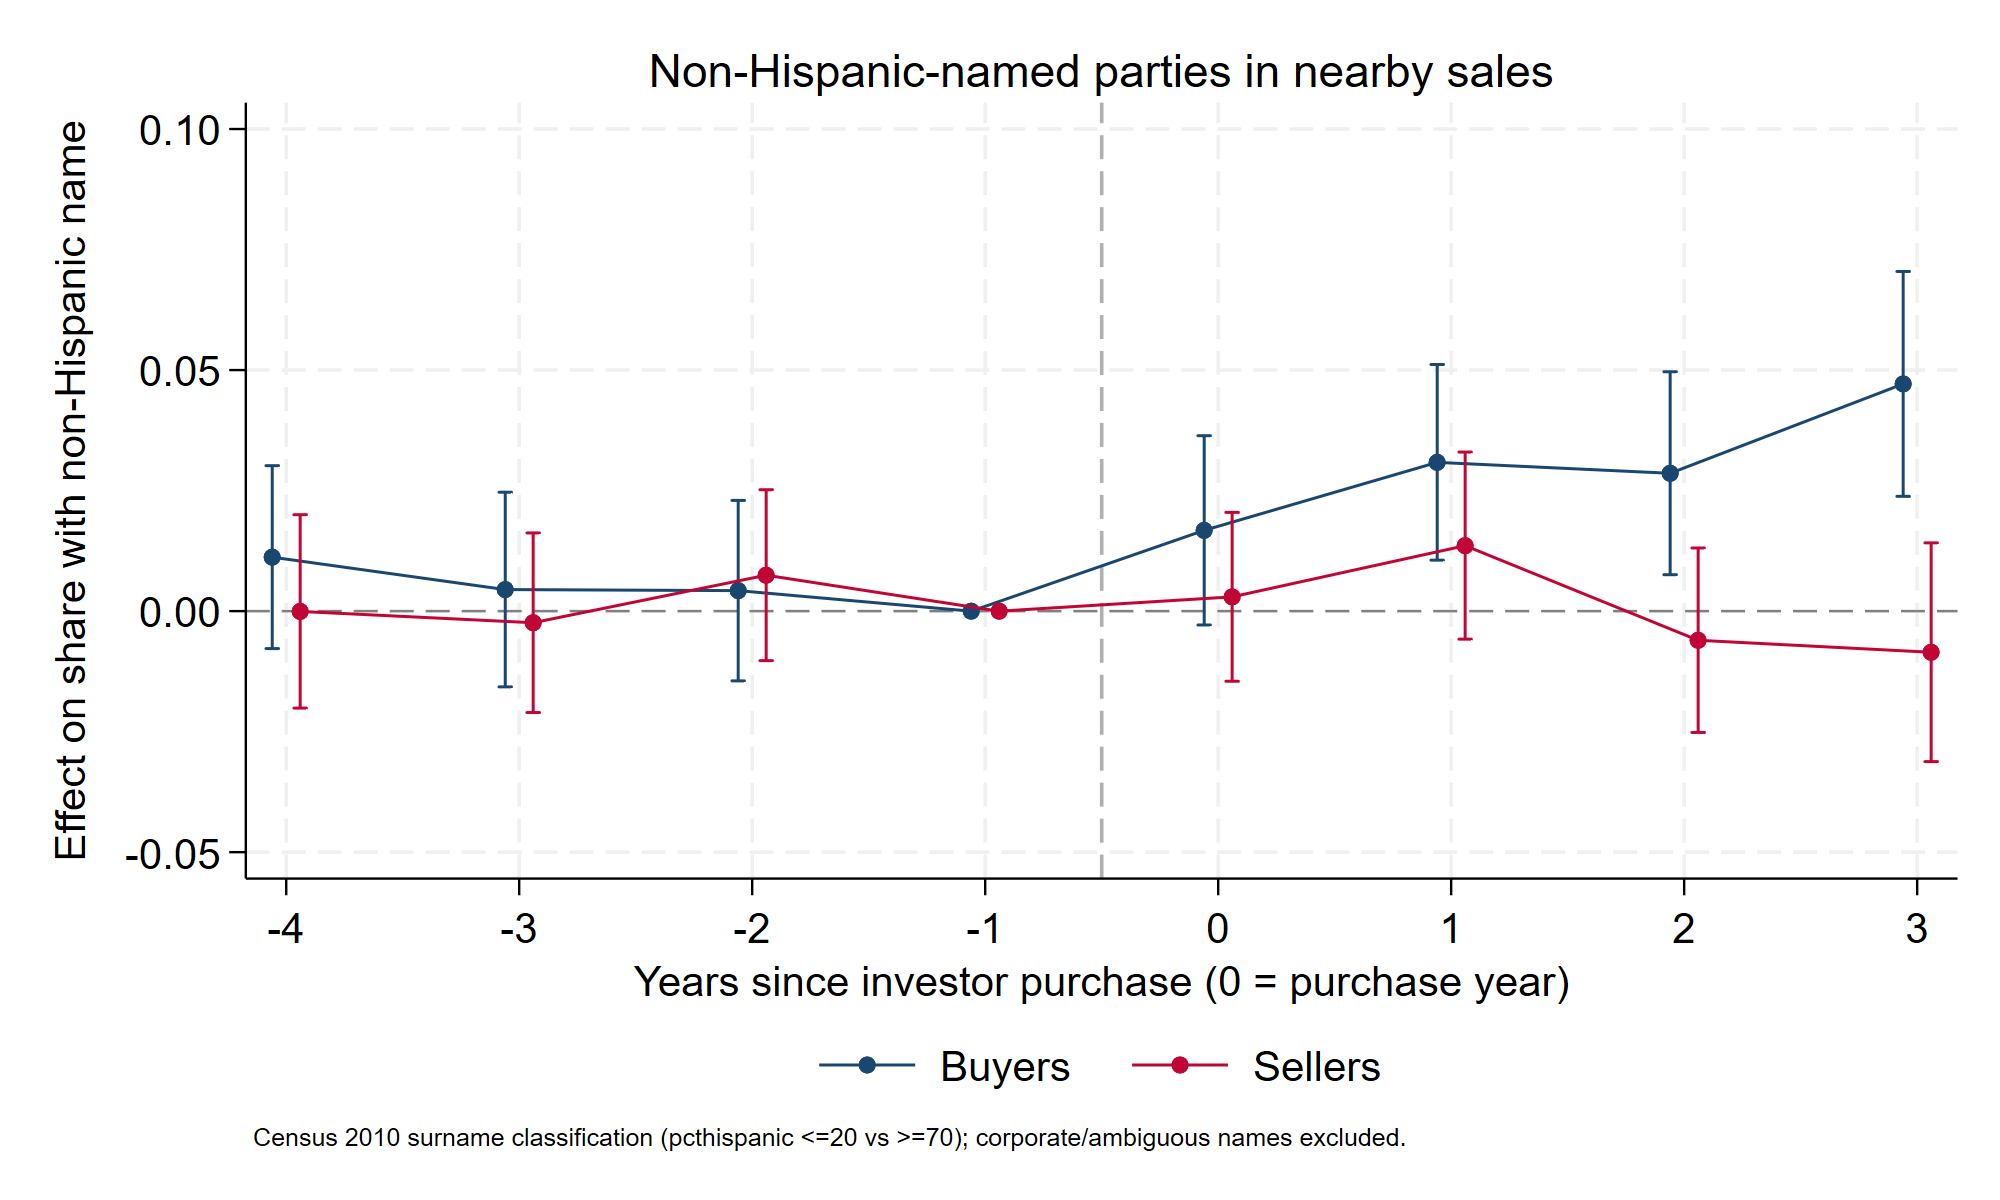
\includegraphics[width=.85\textwidth]{fig7_parties.png}
  \caption{\textbf{Who transacts: buyers vs.\ sellers.} Effects on the share
  of nearby sales with non-Hispanic-named buyers and, separately, sellers
  (Census 2010 surname classification; corporate and ambiguous names
  excluded). Buyer share rising faster than seller share means the area is
  net-importing mainland owners after an investor arrives --- the composition
  shift price indices cannot see.}
  \label{fig:parties}
\end{figure}

\begin{figure}[htbp]
  \centering
  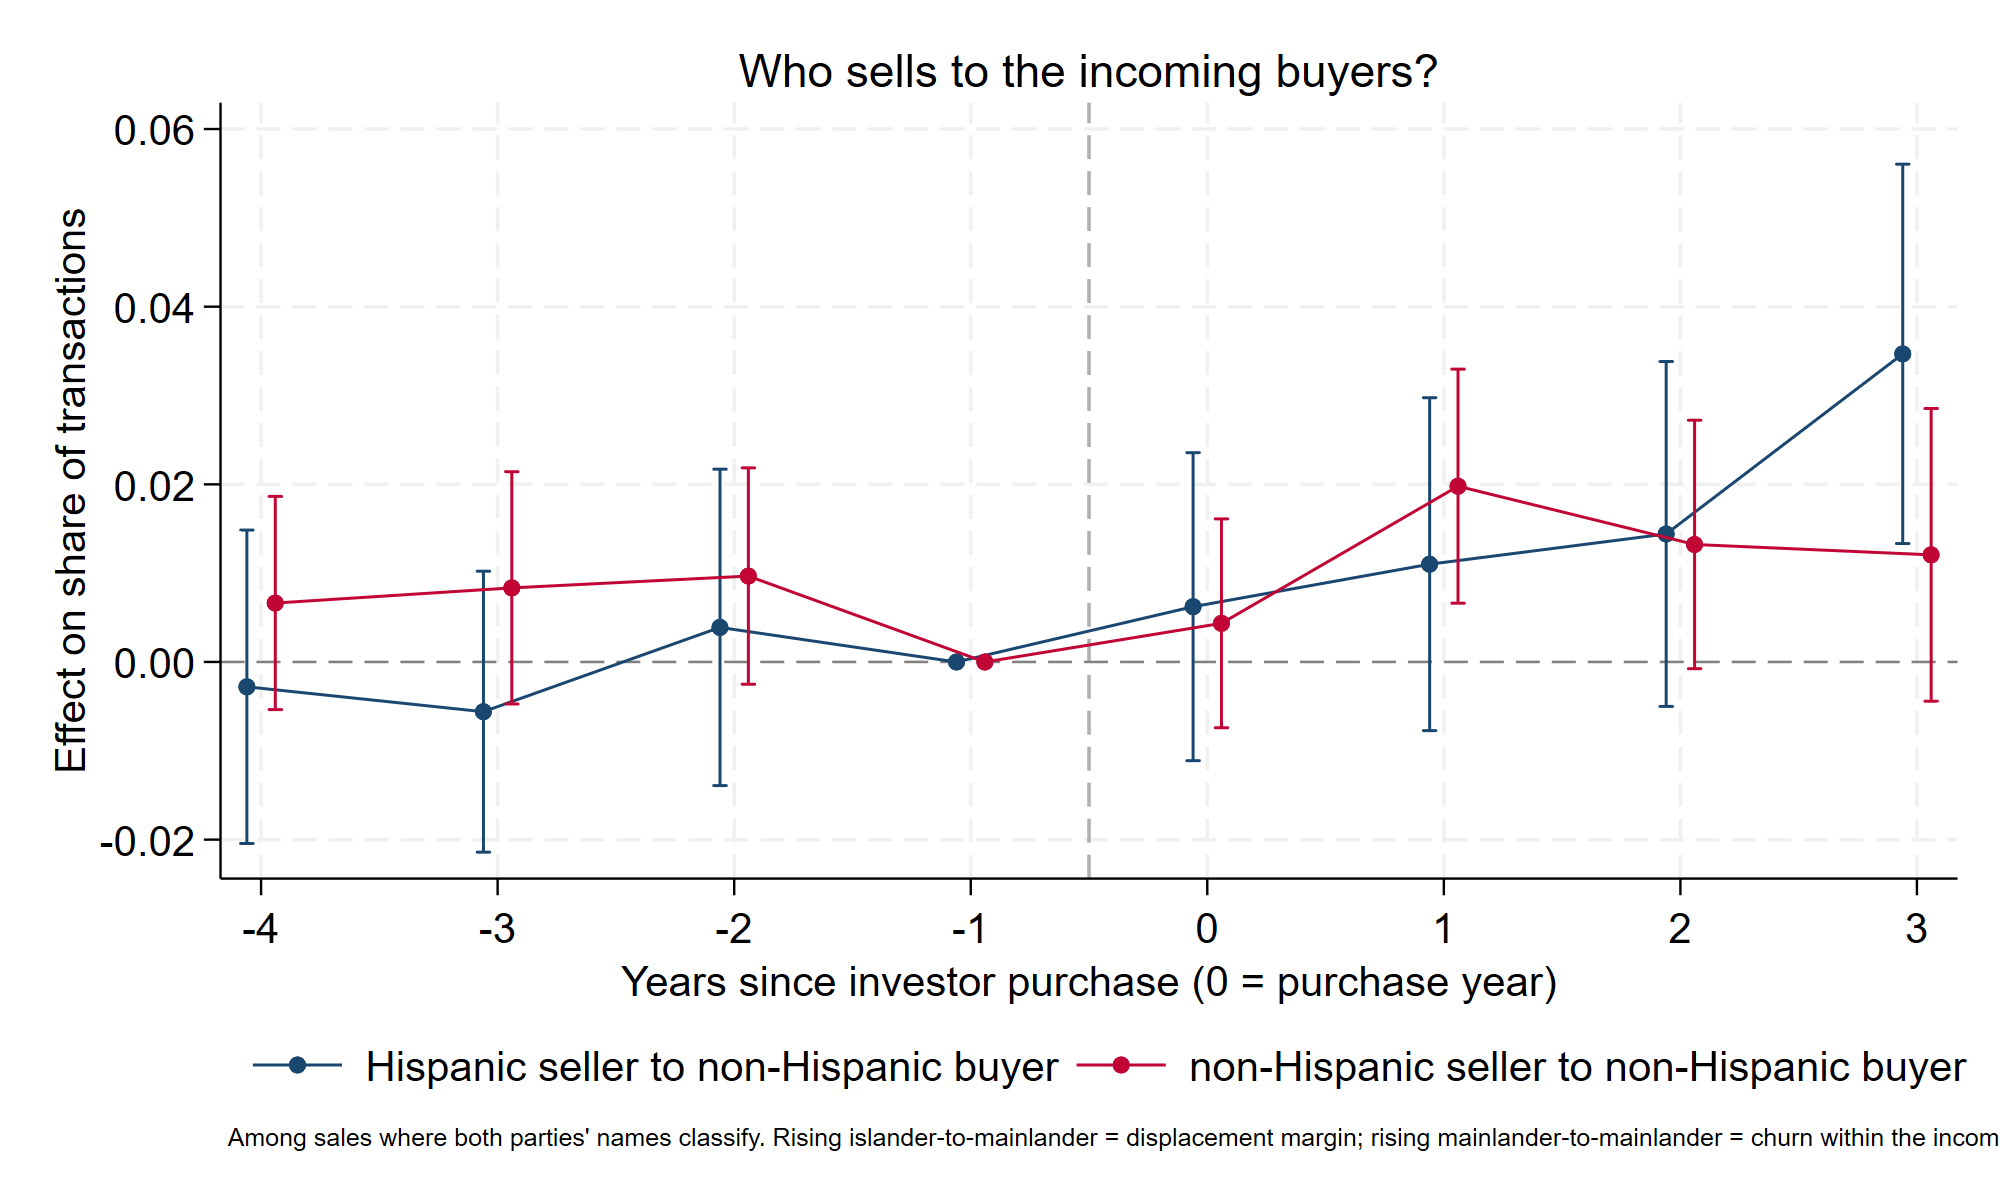
\includegraphics[width=.85\textwidth]{fig8_transitions.png}
  \caption{\textbf{Transition types.} Effects on the shares of transactions
  that are Hispanic-seller$\to$non-Hispanic-buyer versus
  non-Hispanic-seller$\to$non-Hispanic-buyer (among sales where both parties
  classify). Rising islander$\to$mainlander transitions indicate conversion of
  locally held housing to incomers (the displacement margin); rising
  mainlander$\to$mainlander indicates churn within an already-converted
  segment --- together distinguishing ``investors lead conversion'' from
  ``investors cluster where conversion already occurred.''}
  \label{fig:transitions}
\end{figure}

\begin{figure}[htbp]
  \centering
  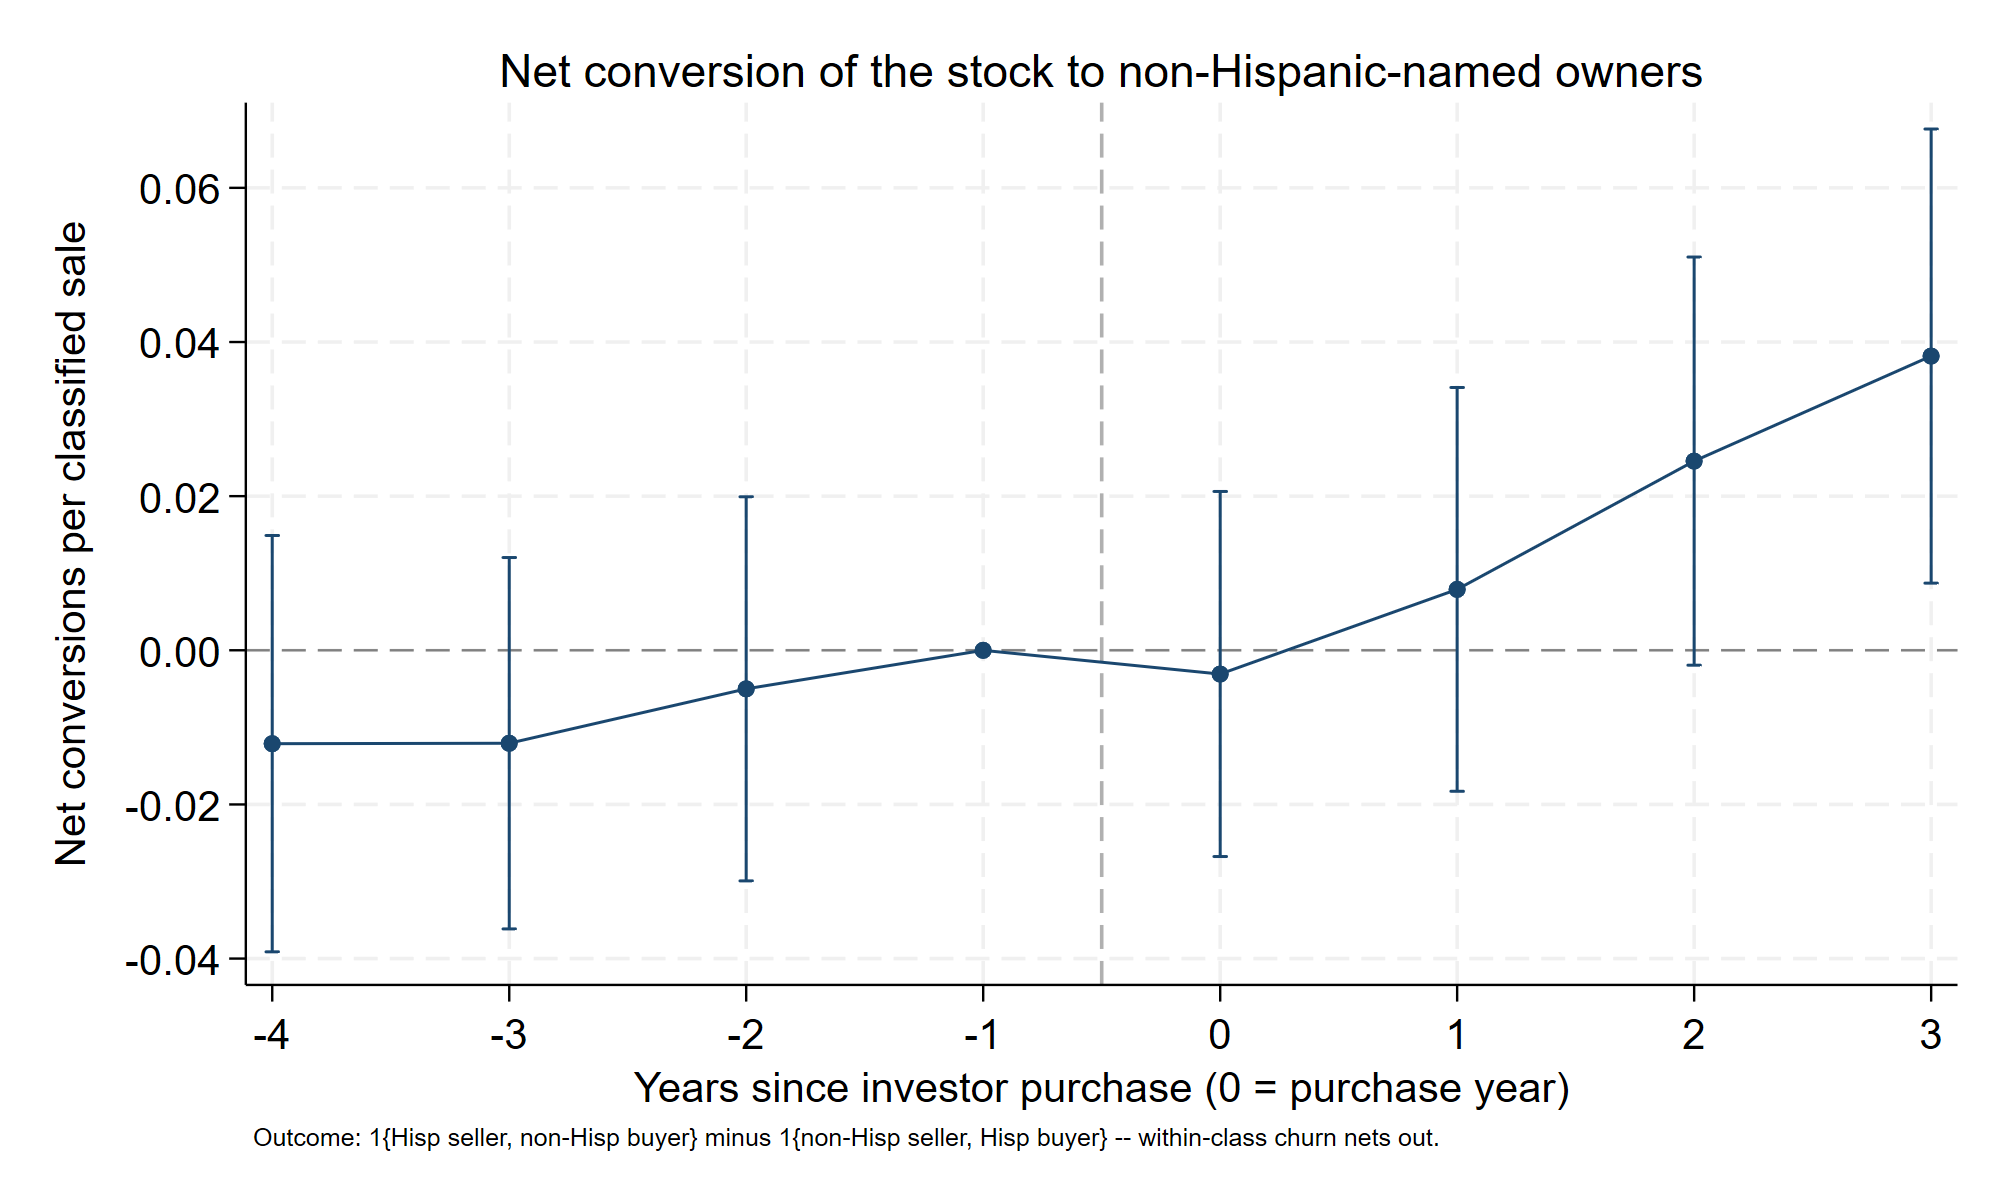
\includegraphics[width=.85\textwidth]{fig8b_netinflow.png}
  \caption{\textbf{Net compositional inflow.} The two transition series
  combined into one displacement measure:
  $1\{$Hispanic seller, non-Hispanic buyer$\}$ minus
  $1\{$non-Hispanic seller, Hispanic buyer$\}$ per classified sale. A sale
  changes the ownership composition of the stock only when the parties'
  classes differ, so within-class churn (including
  mainlander$\to$mainlander resales) nets out; a positive post-event effect
  is net conversion of the nearby stock from Hispanic-named to
  non-Hispanic-named owners. Pre-period flat ($-0.5$pp, s.e.\ $1.0$); the
  net conversion rate rises to $+2.5$pp and $+3.8$pp per sale in years 2--3;
  post$-$pre $+2.4$pp (s.e.\ $0.9$, $p<0.01$) per classified sale.}
  \label{fig:netinflow}
\end{figure}

\clearpage

\section{The tract-level design and reconciliation (Design 2)}
\label{sec:design2}

\subsection{Data and specification}

The tract-level design asks what the ring design structurally cannot: whether
investor purchases move \emph{whole neighborhoods}, including the component
common to treated areas that near--far contrasts difference out. The outcome
panel is the Red Atlas tract$\times$month transaction file (918 of 981
2020-vintage tracts, 2008--2025), aggregated to tract$\times$year with the
annual price defined as the transaction-count-weighted mean of monthly tract
means (composition-noise reduction; the simple mean is a robustness
variant). Treatment timing comes from the dated decree-era events: a tract is
treated from the year of its first identified investor purchase (235 treated
tracts; 1{,}200 events), with never-treated tracts as controls. Estimation is
annual LP-DiD (pre-window 4, post-window 3) on $100 \times \ln(\text{price})$,
with and without county fixed effects.

\subsection{Results}

Prices in treated tracts rise by a pooled $+7.6$ log points
(s.e.\ $1.8$) after the first investor purchase, with flat pre-period
coefficients; adding county fixed effects leaves the estimate unchanged
($+7.5$), and the simple-mean construction gives $+6.1$
(Figure~\ref{fig:tract_es}). Splitting treated tracts by investor
concentration reproduces the dose pattern at tract scale: tracts with five or
more identified purchases (44 tracts) show $+18.3$ ($2.9$), tracts with one
to four show $+3.8$ ($2.1$) (Figure~\ref{fig:tract_dose}). Transaction
\emph{volume} falls in treated tracts, but its pre-period coefficients are
significantly negative, so parallel trends fails for that outcome and we
treat it as descriptive only.

\begin{figure}[htbp]
  \centering
  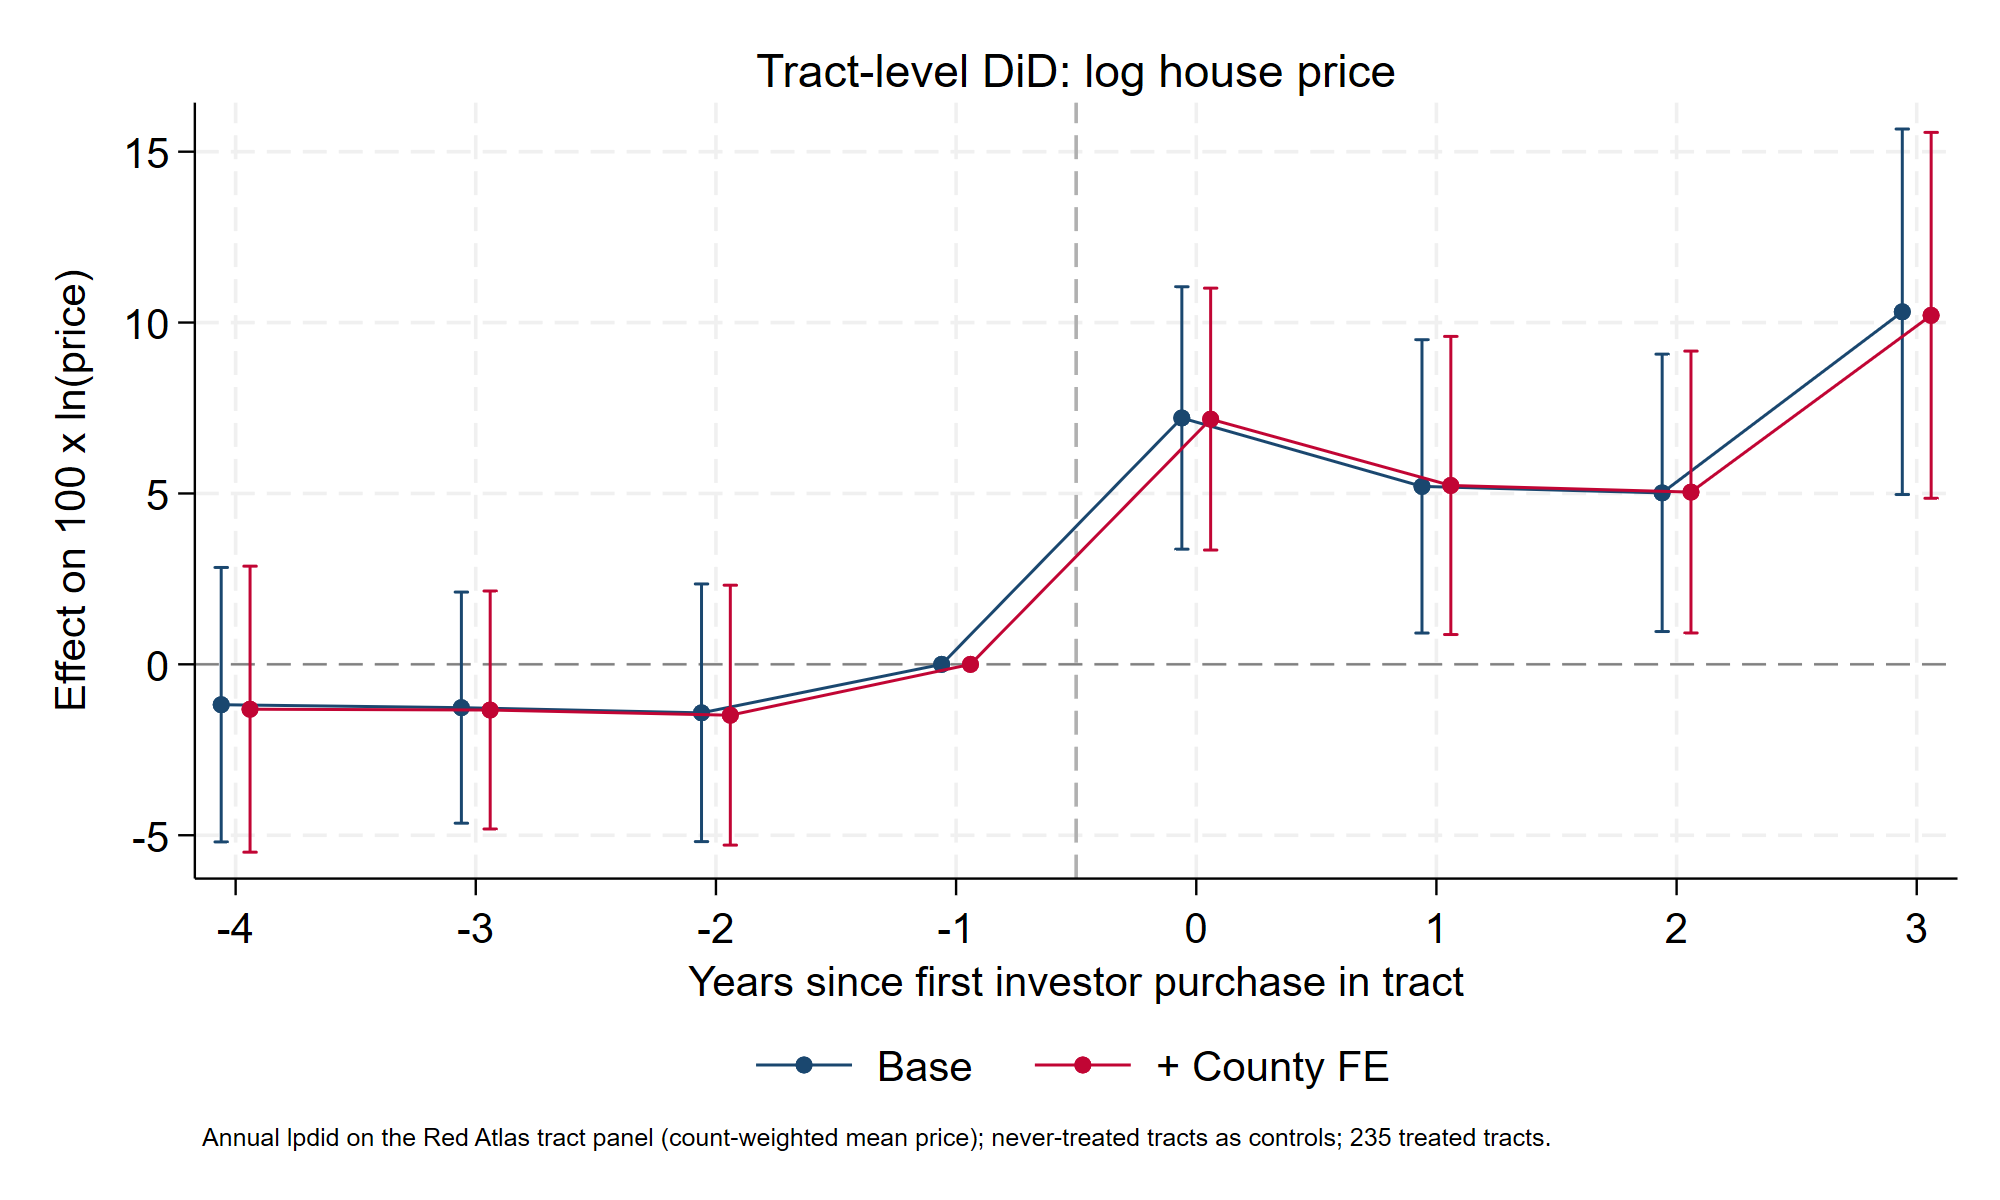
\includegraphics[width=.85\textwidth]{figT1_lnhp_es.png}
  \caption{\textbf{Tract-level event study: log house price.} Annual LP-DiD on
  the Red Atlas panel, 235 treated tracts vs never-treated controls; base and
  county-FE series are indistinguishable and pre-trends are flat.}
  \label{fig:tract_es}
\end{figure}

\begin{figure}[htbp]
  \centering
  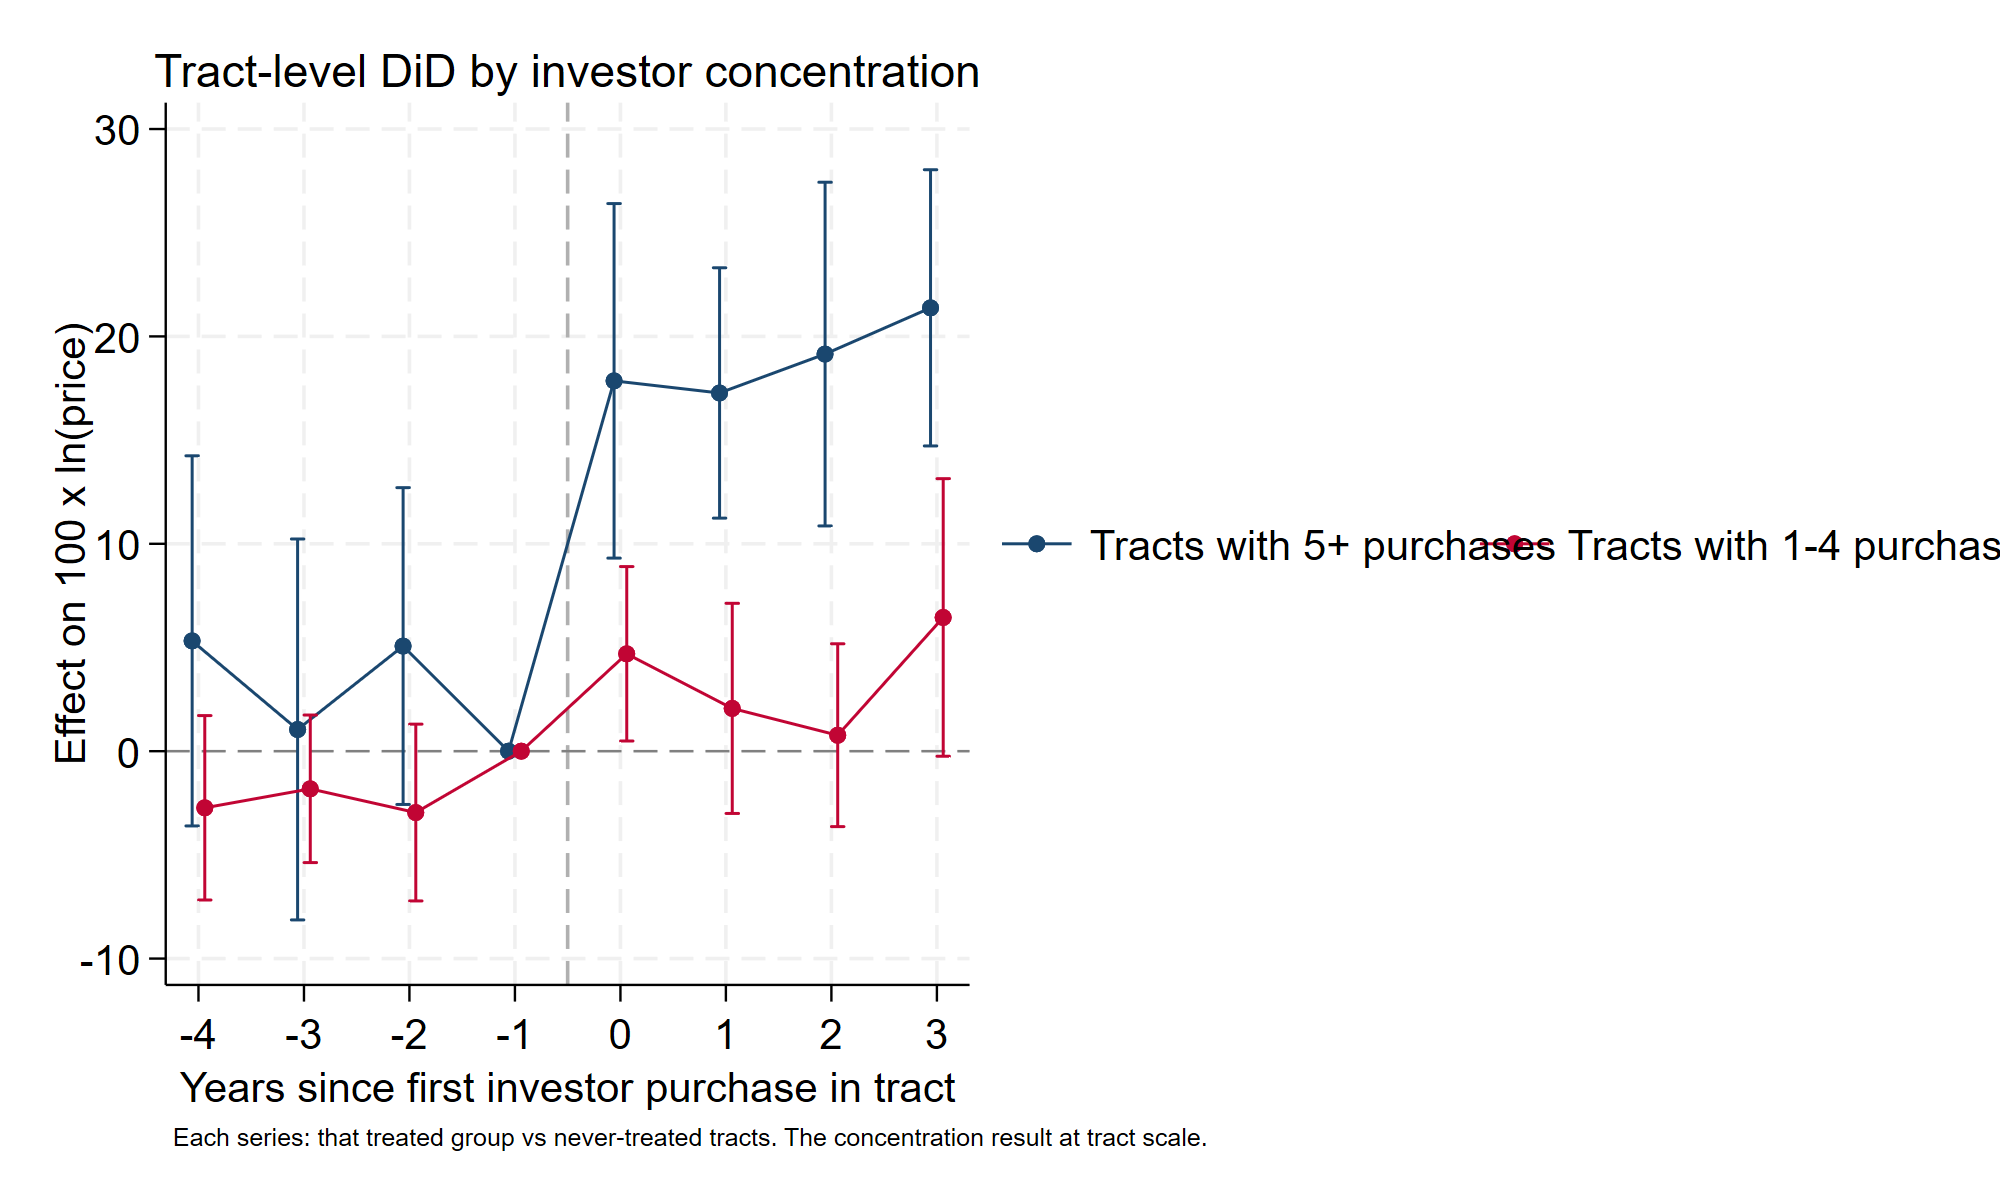
\includegraphics[width=.85\textwidth]{figT2_dose_es.png}
  \caption{\textbf{Tract-level event study by investor concentration.} Tracts
  with 5+ identified purchases versus tracts with 1--4, each against
  never-treated controls: the concentration result at tract scale.}
  \label{fig:tract_dose}
\end{figure}

\subsection{Reconciliation: the whole vs the sum of the parts}

Because the ring design delivers a distance gradient, it implies a
\emph{prediction} for each treated tract: the stock-value-weighted average of
$\beta(d)$ over the tract's parcels --- the tract-level effect if
micro-spillovers were the whole story. Comparing observed tract-DiD estimates
to these predictions decomposes the aggregate
(Figure~\ref{fig:reconciliation}): tracts with 1--4 purchases sit at or below
their prediction (observed $+3.8$ vs predicted $+5.4$) --- micro-spillovers
fully account for them --- while the 44 concentration tracts exceed their
prediction by roughly 11 log points (observed $+18.3$ vs predicted $+7.5$).
A market-level channel beyond proximity operates only where investors
concentrate.

\begin{figure}[htbp]
  \centering
  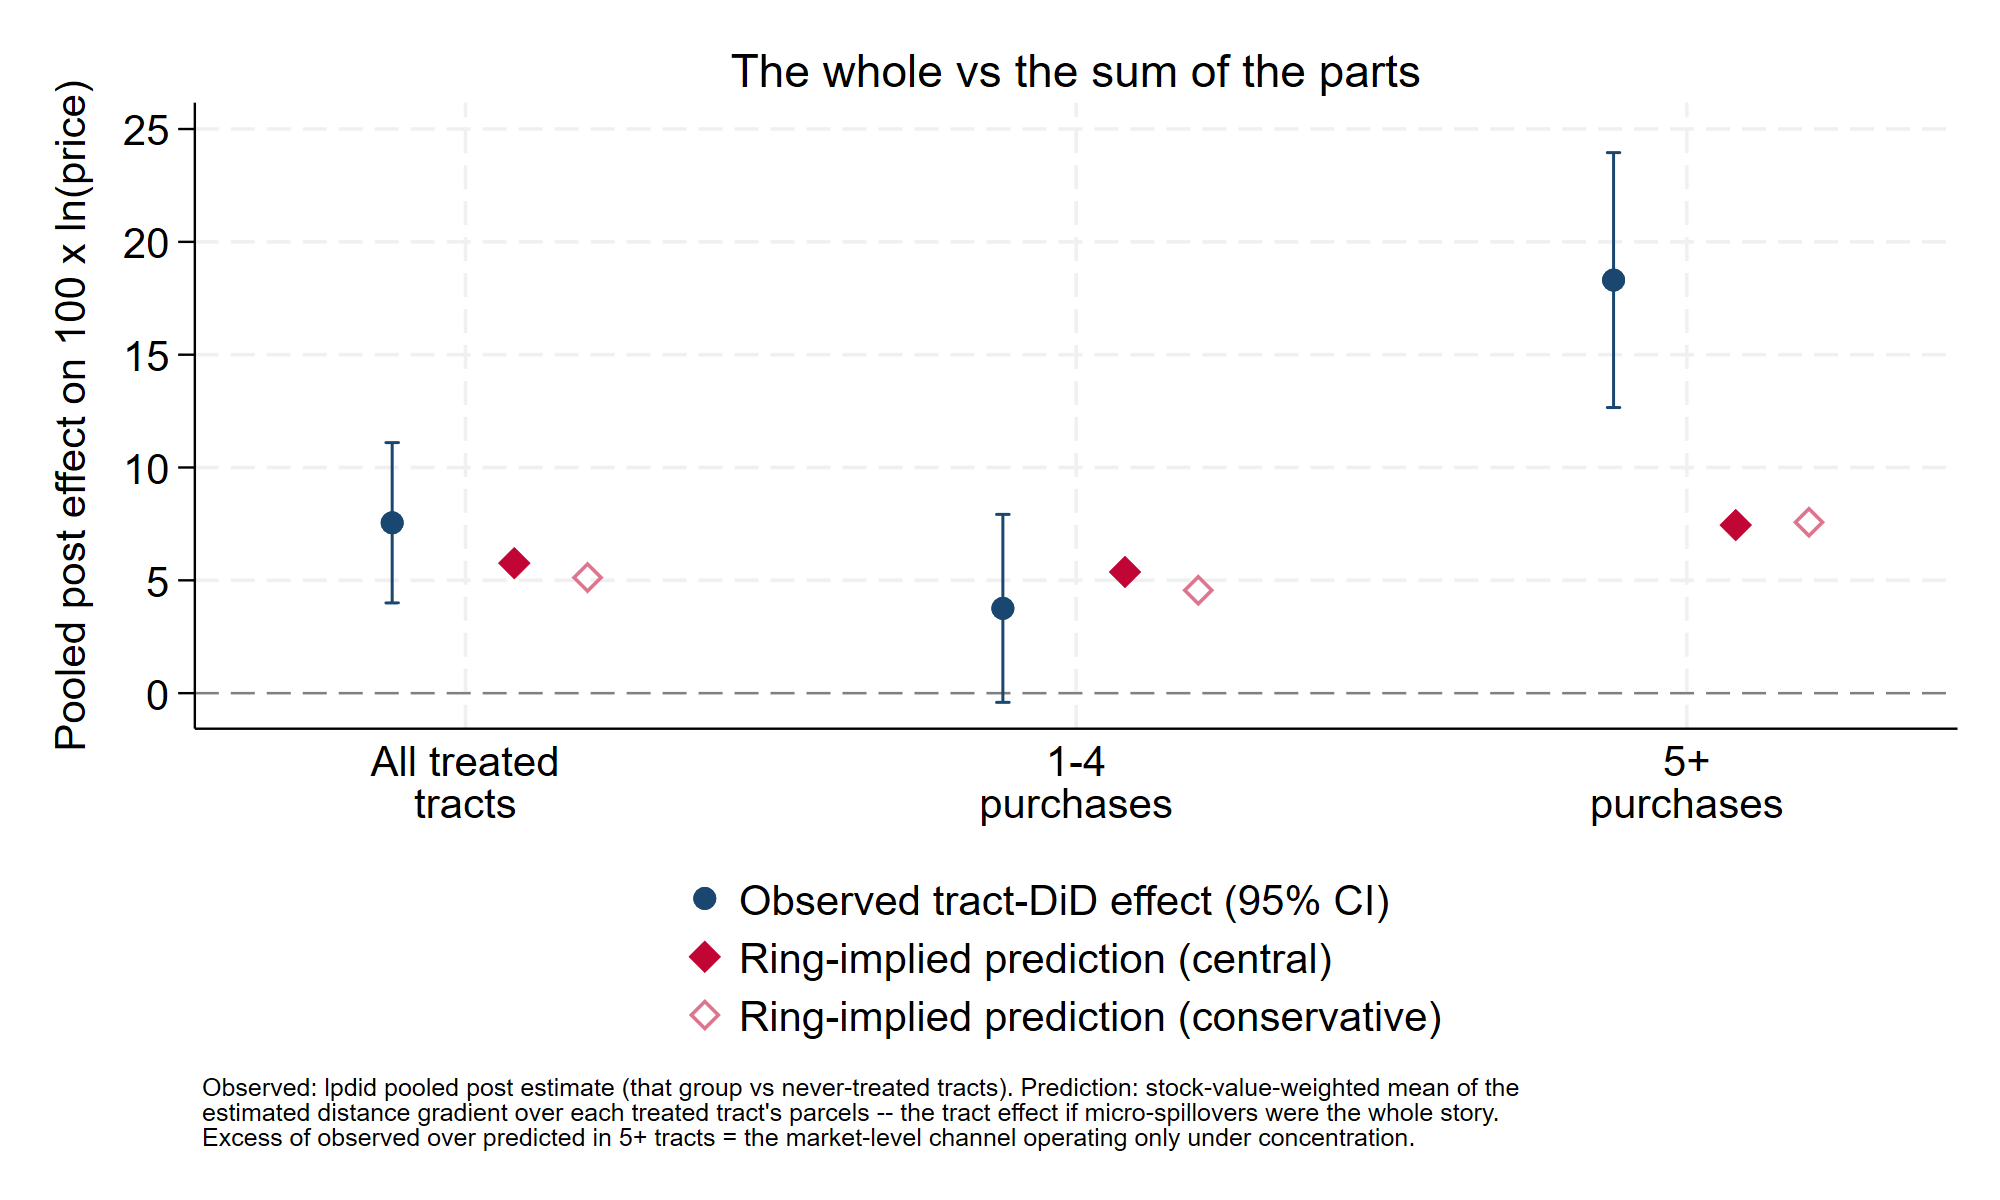
\includegraphics[width=.85\textwidth]{figT4_reconciliation.png}
  \caption{\textbf{Observed tract effects vs ring-implied predictions.}
  Observed: LP-DiD pooled post estimates by dose group. Predictions:
  stock-value-weighted distance-gradient effects over each treated tract's
  parcels. The all-treated and 1--4-purchase groups sit on their predictions;
  the 5+ group's excess ($\approx$11 log points) is the concentration
  channel.}
  \label{fig:reconciliation}
\end{figure}

\subsection{Aggregation}

Integrating the estimated gradient over the exposure distribution of the
island's improved housing stock (60.0\% of parcels, 63.1\% of assessed value,
lie within 2.5\,km of an identified event) yields an island-wide average
price effect of $+2.1$ to $+3.0$\%, or \$6.3--8.0B of housing value at
band-specific market/assessed ratios --- roughly 6--8\% of Puerto Rico's
post-2019 boom (FHFA purchase-only index: $+64$\% 2019--2024). Adding the
concentration excess in the 44 high-dose tracts ($\approx$\$4.3B) raises the
identified program footprint to $\approx$\$11--12B, about 10--11\% of the
boom. At municipio level, using municipio repeat-sales indices as the local
boom denominators, footprints in the top investor municipios are much larger:

\begin{center}
\small
\setlength{\tabcolsep}{4.5pt}
\begin{tabular}{lrrrrrrrrr}
\toprule
 & \multicolumn{2}{c}{Local boom '19--'24} & &
   \multicolumn{2}{c}{Synthesis} & \multicolumn{2}{c}{Ring design} &
   \multicolumn{2}{c}{Tract DiD} \\
\cmidrule(lr){2-3} \cmidrule(lr){5-6} \cmidrule(lr){7-8} \cmidrule(lr){9-10}
Municipio & Growth & \$ & Uplift & Total & 5+ diff. & Total & 5+ tracts & Total & 5+ tracts \\
\midrule
Rinc\'on     & $+148\%$ & \$1.1B  & \$0.34B & 31.1\% & 17.7\% & 13.4\% & 12.7\% & 30.7\% & 30.4\% \\
Dorado       & $+177\%$ & \$3.7B  & \$0.97B & 25.9\% & 14.4\% & 11.5\% & 10.3\% & 25.0\% & 24.8\% \\
San Juan     & $+89\%$  & \$17.8B & \$4.29B & 24.1\% &  9.0\% & 15.1\% &  6.0\% & 17.8\% & 15.1\% \\
R\'io Grande & $+115\%$ & \$2.0B  & \$0.48B & 24.0\% & 15.7\% &  8.4\% &  6.1\% & 23.5\% & 21.8\% \\
Carolina     & $+91\%$  & \$7.6B  & \$1.32B & 17.2\% &  6.8\% & 10.4\% &  4.7\% & 12.2\% & 11.6\% \\
Guaynabo     & $+124\%$ & \$5.4B  & \$0.84B & 15.5\% &  2.3\% & 13.2\% &  1.7\% &  8.6\% &  4.0\% \\
Humacao      & $+121\%$ & \$2.5B  & \$0.39B & 15.5\% &  7.2\% &  8.3\% &  5.1\% & 13.7\% & 12.4\% \\
\bottomrule
\end{tabular}
\end{center}

\noindent All columns share one valuation convention: each parcel at assessed
value times its tract's median market/assessed ratio (2019+ sales; municipio
and island fallbacks). The dollar boom is the municipio's market stock times
$1-1/(1+g)$, the portion of current value attributable to repeat-sales growth
$g$ since 2019; Uplift is the synthesis in dollars. Shares of boom connect
exactly: \emph{Ring, Total} integrates the distance gradient over all parcels
and \emph{5+ tracts} restricts to parcels in 5+-purchase tracts; \emph{Tract
DiD} applies the dose-specific tract effects to treated-tract stock
(\emph{Total}: all treated tracts; \emph{5+ tracts}: the high-dose subset).
The synthesis \emph{5+ differential} is Tract DiD (5+) minus Ring (5+) ---
the tract-wide repricing beyond what proximity predicts --- and
\emph{Synthesis, Total} $=$ Ring (Total) $+$ the 5+ differential, so the ring
layer is never double-counted.

All aggregates are lower bounds: exposure counts only the 1{,}200
name-identified purchases, excluding LLC and unmatched investors; the
capitalization step applies transaction-price effects to the full stock; and
event effects predating 2019 enter the numerator while the boom clock starts
in 2019.

\subsection{Mortgage originations: volumes are a convincing null}

HMDA loan-level data for Puerto Rico (2018--2024; 105{,}559 originations,
aggregated to 2020-vintage tract$\times$year) show no detectable response of
mortgage lending in treated tracts: Poisson (PPML) estimates with tract and
year fixed effects are statistically zero for owner-occupied purchases
($-0.5$\%, s.e.\ $5.4$), non-owner-occupied purchases ($+3.0$\%, $11.3$),
rate/term and cash-out refinancings, and total originations, and are
unchanged with county$\times$year fixed effects. Consistent with decree
investors transacting predominantly in cash, the program's effects appear in
prices and buyer composition rather than local credit expansion.

\subsection{Who can still buy: borrower composition in treated tracts}

Splitting purchase originations by HMDA's self-reported borrower ethnicity
(Hispanic or Latino vs.\ not; joint and unavailable excluded) sharpens the
displacement interpretation. Since decree investors buy in cash, HMDA is
effectively a census of the \emph{financed} --- overwhelmingly local, 94.6\%
Hispanic --- side of the market. To get adequate pre-periods we extend the
panel back to 2012 using CFPB's historic HMDA files, on a population that is
consistent across the 2017/2018 reporting change: originated first-lien,
owner-occupied, 1--4 family home-purchase loans (2012--2024; annual
volumes are smooth across the seam). Three results
(Figures~\ref{fig:hmdainc}--\ref{fig:hmdaincdose}). First, borrower
\emph{income} rises after treatment --- pooled $+9.6$\% (s.e.\ $1.9$),
reaching $+10.0$\% at $h\!\ge\!3$ --- and with up to six pre-years of data
(displayed with the endpoint binned at $-4$) the pre-period is now flat
($-3.7$, $-1.1$, $-2.4$, individually and jointly insignificant, with no
run-up into treatment; the apparent pre-drift in the short 2018--2024 panel
was an artifact of its truncated window).
Second, the income shift is concentrated where investors concentrate:
$+17.6$\% (s.e.\ $4.9$) in 5+-purchase tracts vs.\ $+7.9$\% (s.e.\ $2.0$)
in 1--4-purchase tracts. Third, on the extensive margin, Hispanic-borrower
purchase counts are unchanged (pooled $+0.6$\%, s.e.\ $4.5$) while
\emph{non-Hispanic} borrower purchases rise $+37$\% (s.e.\ $14$) from a thin
base --- financed mainlander entry is now detectable, not just cash entry.
Together: local buyers as a group keep transacting, but the marginal
financed buyer moves up the income distribution, most strongly in high-dose
tracts --- the affordability-displacement margin, measured on self-reported
ethnicity and income rather than the surname proxy.

\begin{figure}[htbp]
  \centering
  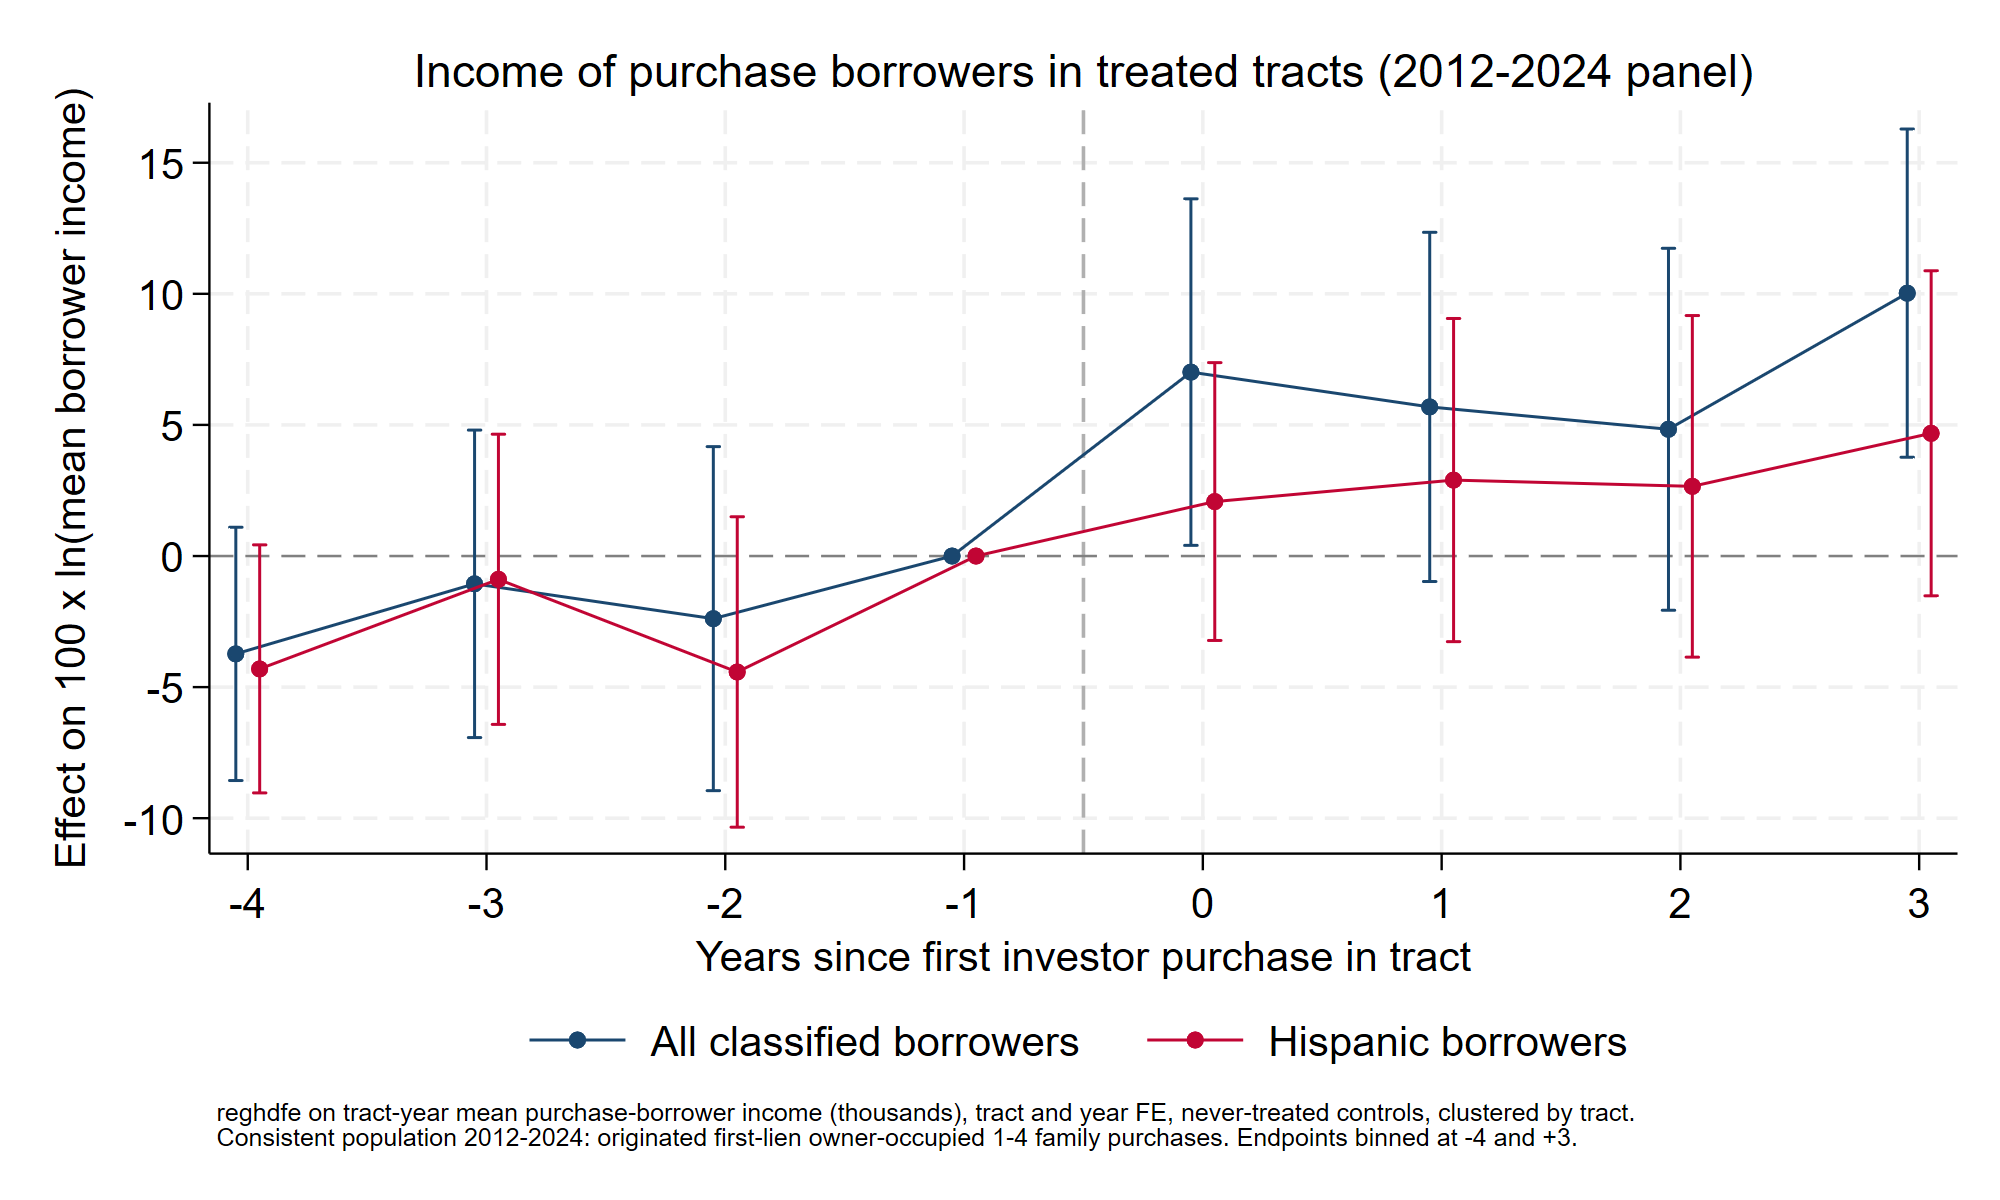
\includegraphics[width=.85\textwidth]{../design2/figH7_income_long.png}
  \caption{\textbf{Income of purchase borrowers, 2012--2024 panel.} Effect on
  $100\times\ln$(mean borrower income) among first-lien owner-occupied
  purchase originations in treated tracts; all classified borrowers and
  Hispanic borrowers only. No pre-trend (endpoint binned at $-4$ pools
  horizons back to $-6$); pooled $+9.6$\% (s.e.\ $1.9$).}
  \label{fig:hmdainc}
\end{figure}

\begin{figure}[htbp]
  \centering
  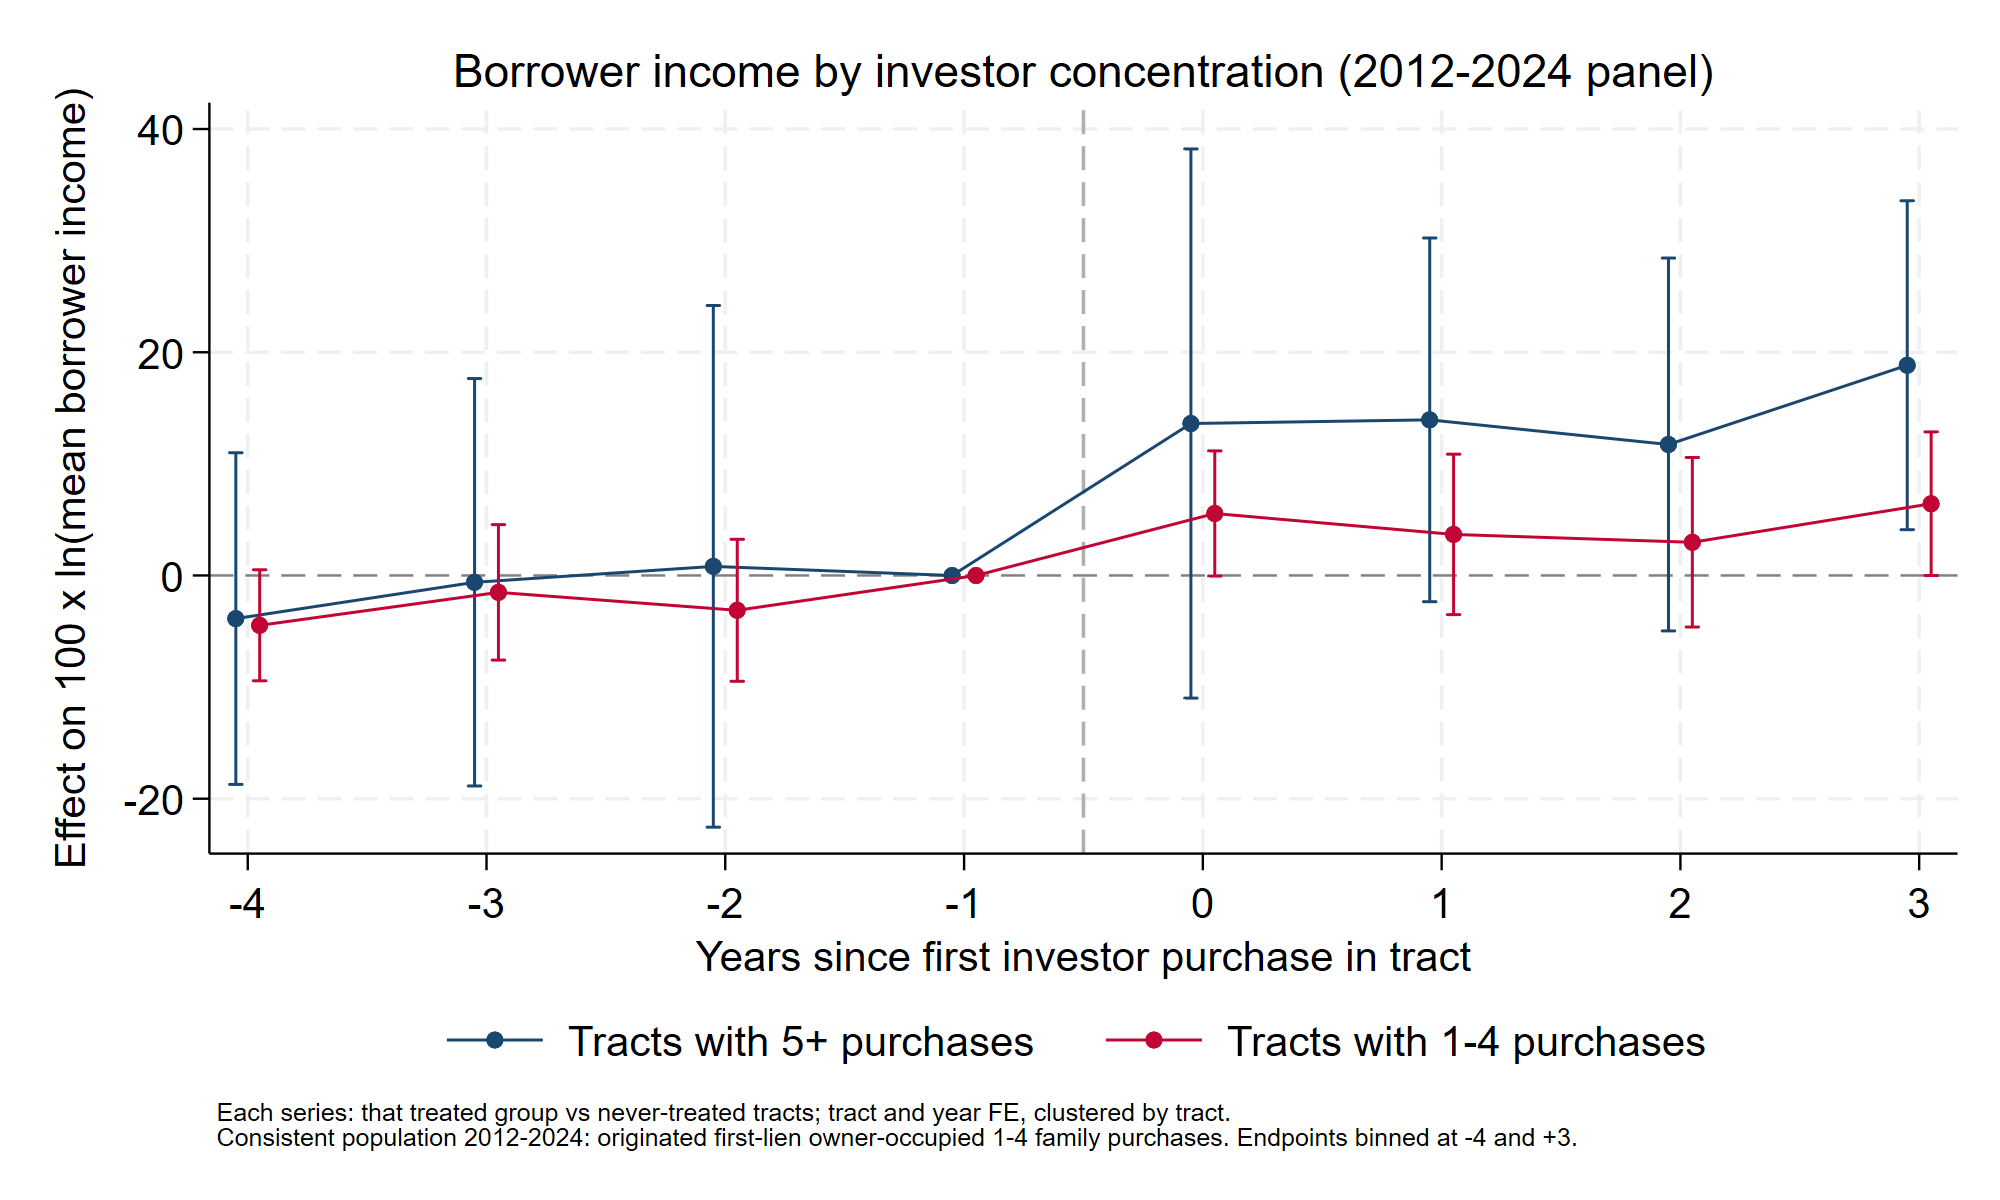
\includegraphics[width=.85\textwidth]{../design2/figH8_income_dose_long.png}
  \caption{\textbf{Borrower income by investor concentration, 2012--2024
  panel.} Each series: that treated group vs.\ never-treated tracts. The
  income shift is twice as large in 5+-purchase tracts ($+17.6$\%, s.e.\
  $4.9$) as in 1--4-purchase tracts ($+7.9$\%, s.e.\ $2.0$) --- the same
  concentration gradient as prices.}
  \label{fig:hmdaincdose}
\end{figure}

\section{Standing caveats}

\begin{enumerate}[leftmargin=*]
  \item \textbf{Last-sale censoring} (CRIM): pre-period sales are survivors
  that never resold; addressed by design and Figure~5.
  \item \textbf{Site selection}: investors choose appreciating micro-areas;
  estimates are local spillovers \emph{conditional on} location choice, not
  ``the effect of the Act.''
  \item \textbf{Match selection}: identified investors skew toward
  single-property, personal-name buyers; entity (LLC/trust) purchases are
  missing.
  \item \textbf{Name proxy}: understates mainland presence; corporate and
  ambiguous names are excluded from shares.
  \item \textbf{Assessed values} are on CRIM's 1957 basis --- valid as
  cross-sectional controls and composition outcomes, never as market values.
\end{enumerate}

\end{document}
